\chapter{Differential networks reveal the dynamics of animal pests and disease co-occurrences}

\subsection{Introduction}
Rice \textit{Oryza sativa}) is a major crop in South and Southeast Asian. Generally, rice farmers cultivate 2 rice crops per year, with the typical seasonal crop cycles or rotations being rice-rice-fallow or rice-rice-secondary crops (corn, soybean, peanut). The Food and Agriculture Organization of the United Nations (FAO) estimates that approximately 70 percent of total lowland rice area produces 2 rice crops each year. The first crop is cultivated in the wet season, while another is in the dry season. The important role of seasonal cropping in the temporal dynamics of animal pests and diseases has been studied under farmers field survey in South and Southeast Asia by the use of multivariate techniques \citet{Savary_2000_Characterization, Willocquet_2008_Simulating}. The previous studies showed that Injuries profiles (the combination of injuries) differ from season to season in term of weather pattern. In the dry season, crop losses were lower than in the wet season. A previous study based on surveys done in farmers’ rice fields in the region of lowland rice were shown to be strongly associated with injury profiles.
In the previous chapter, the co-occurrence networks to yield co-occurrence networks, a methodological approach which has already proved fruitful in a variety of different applications.  Plant injuries caused by pests maybe affect yield production. Therefore, in this chapter, I attempted to characterize the patterns of rice injuries by studying the changes in the co-occurrence patterns of rice injuries (textit{e.g} disease incidence, animal pest injury incidence) at different yield levels.


Differential network analysis aims to compare the connectivity of two nodes at 2 different conditions. As demonstrated by several studies, differential networks can identify important nodes implicated in my fields, and also provide critical novel insights not obtainable using other approaches. In this work, I explore the the properties of network of a complex association of rice injuries at different yield levels. Elucidating the rice injuries association represents a key challenge, not only for achieving a deeper understanding of injury association (injury profiles) but also for identifying the unique association. Given that the injury association is governed by a complex network of injuries association, it seems natural to explore network properties which may help elucidate some of different association presenting in the different seasons.

My overall objective was to identified different co-occurrence patterns at different condition.

explored the relation between local differential association and discuss the meaning of the results in the context of the crop health management, and discuss the potential implications of our findings for development of pest management with a view to future studies.



South and Southeast Asia represents rice growing areas where rice is grown under so diverse soil and climatic conditions. Comparing the topological properties of the nodes associated with rice injuires in different production season and examining the network level topological feature provide us with insight into variation in the co-occurence patterns  this successional climatic. This approach helps contestial  Specifically, I address tge following question: Do the co-occurece network vary between differret production season ? (ii) Do the co-occurence network vary between differnt yield levels.(iii)   To answer these question, I perform co-occurence analyssi to examin the topological feature dynamic across production season, and production enviroments.

ideal continental scale system to explore a complete vegetation gradient from tropical forest to arctic tundra. 

Comparing the topological properties of the nodes associated with forest soil in different climatic regions and examin- ing network-level topological features can provide us with insight into variations in the co-occurrence patterns along this successional climatic gradient. This approach helps contextualize microbial bio- geography by taking into account the complex network of potential interactions among microbes in these environments. Specifically, we addressed the following questions: (i) Do the topological features of co-occurrence network vary between different climate regions? (ii) Do microorganisms from different kingdoms (bacteria, archaea, fungi) exhibit different co-occurrence patterns? (iii) What environmental factors correlate with variation in the topological features of interaction networks? To answer these questions, we performed ribosomal RNA amplicon sequencing analyses on natural, undisturbed forest soil microbiota spanning five successional climate regions and implemented co- occurrence network analysis to examine the topolo- gical feature dynamics across this continental scale. 

Our main objective was to characterize and better understand co-occurrence network patterns in soil microbial communities.

\subsection{Materials and Methods}


\textbf{Calculation of differential correlations}

Fisher's $z$-test was used to identify significant differences between 2 correlations, based on its stringency test and its provision of conservative estimates of true differential correlations among molecules between 2 conditions in the survey data data. 


For the pair of $x_{i}$ injury and $y_{i}$ variable, I denoted the correlation coefficient based on Spearman's correlation coefficient by $c_{xy}^1$ and $c_{xy}^2$ in networks 1 and 2, respectively. To test whether the 2 correlation coefficients were significantly different of each network, I used Spearman's correlation coefficients, the $p$-values of the correlation test, the difference of the 2 correlations, the corresponding $p$-values, and the result of Fisher's z-test. First, I applied the Fisher $z$-transformation in order to stabilize variances due to sample size.

\begin{equation}
\label{eq:zvalue}
z_{xy} = \frac{1}{2} \log\left[{\frac{1 + c_{xy}}{1 - c_{xy}}}\right]
\end{equation}

if we let $z_{xy}^D $ and $z_{xy}^W$ denote the $z$- transformation for dry and wet season variable pairs, respectively.

Next, The $p$- value of the difference in Zf values was calculated
using the standard normal distribution. differences between the two correlations can be test using following. 

\begin{equation}
\label{eq:pofz}
P(Z\geq \left | \frac{z_{xy}^1 - z_{xy}^2}{\sqrt{\frac{1}{N_{1}-3}+ \frac{1}{N_{2}-3}}} \right |
\end{equation}

$N_{D}$ and $N_{W}$ represent the sample size for each of season network for each country. The $Z$ has an approximately Gaussian distribution under null hypotheses that the population correlations are equal. The pair-wise correlation significants are considered at $p$vlaue < 0.05.

\textbf{objective1}

\begin{equation}
A_{diff} = \left\{\begin{matrix}
 1 & \text{when } C_{xy}^D > C_{xy}^W \text{ at } P_{z_{xy}} \text{-value}  < 0.05  \\ 
 0 & \text{when } P_{z_{xy}}  \text{-value}  > 0.05                              \\ 
-1 & \text{when } C_{xy}^W > C_{xy}^D \text{ at } P_{z_{xy}} \text{-value}  < 0.05 
\end{matrix}\right.
\end{equation}


\begin{figure}
\centering
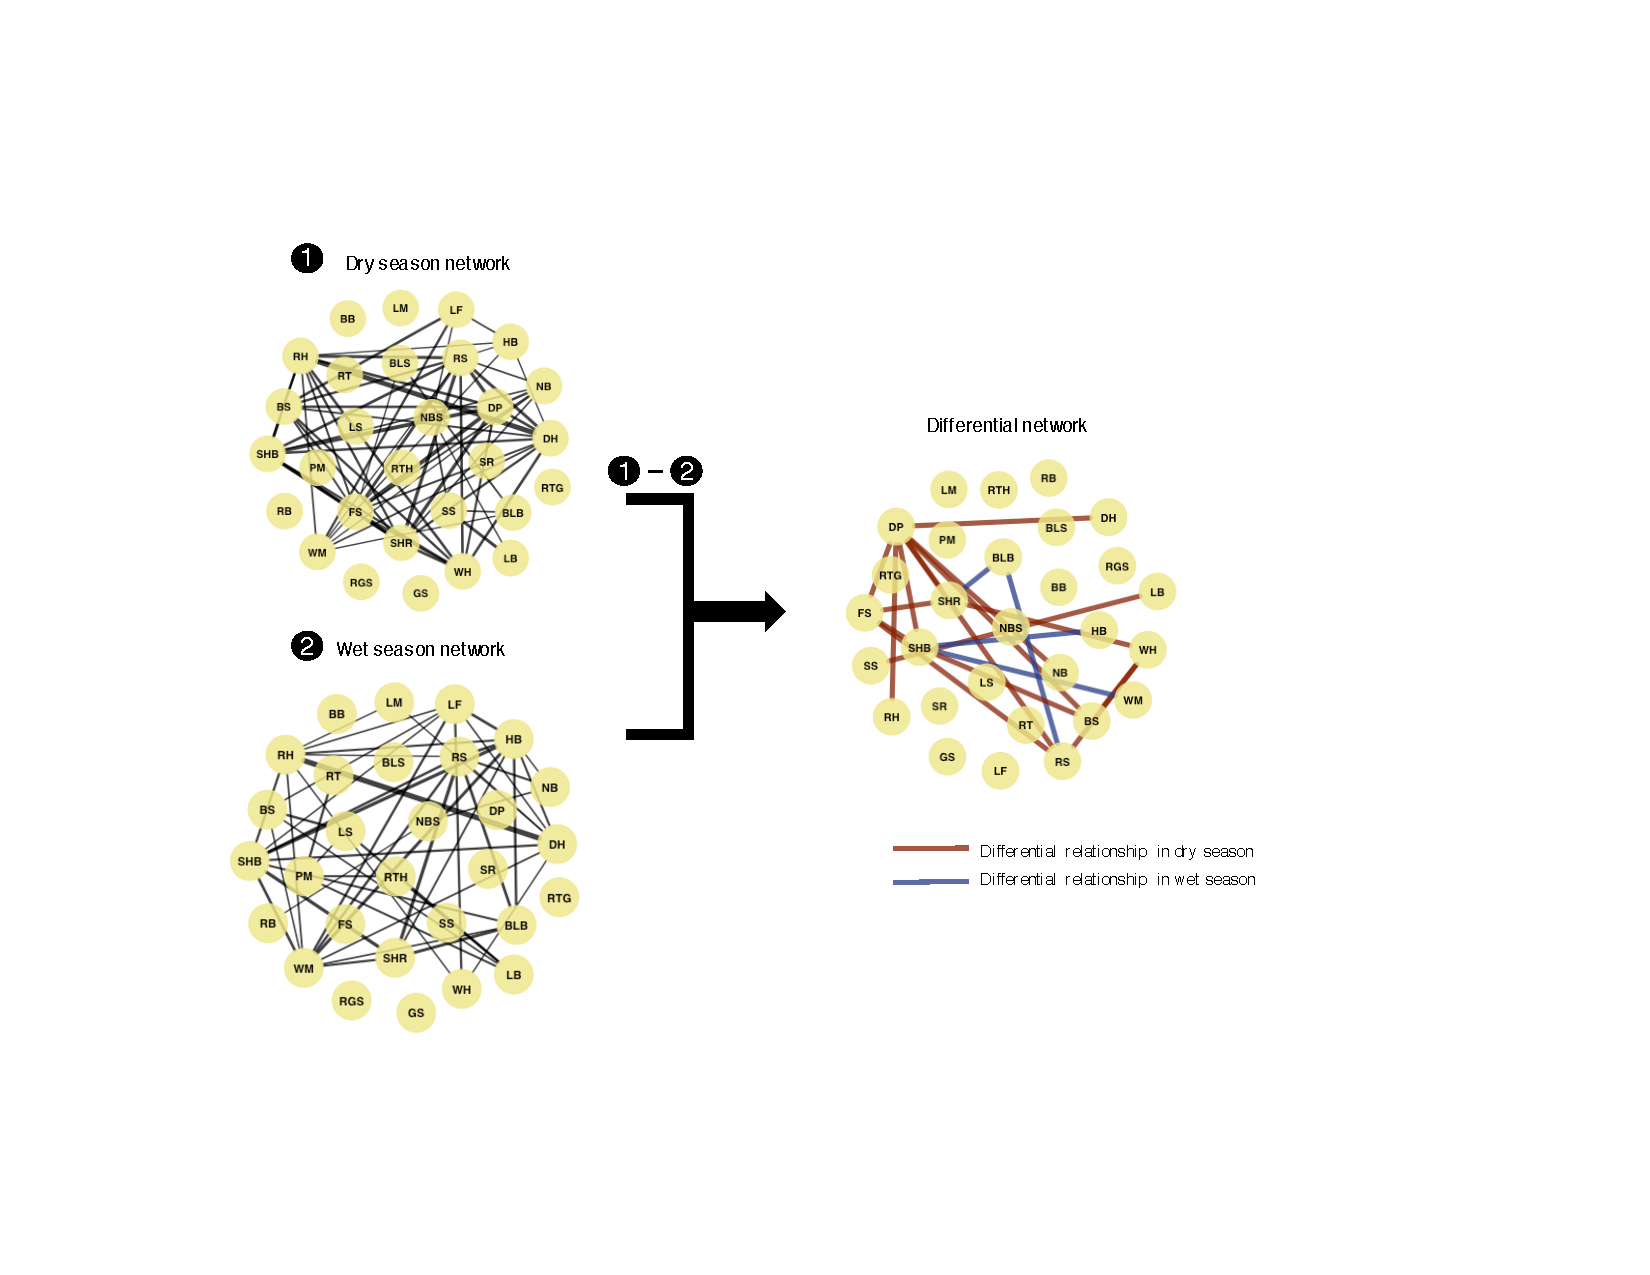
\includegraphics[width = 0.8\textwidth]{figures/pipeline3.pdf}
\caption{Schematic showing principle of differential analysis. Static interaction network are measured in each of two seasons (left) resulting in interactions (black). Dry season is subtracted from wet season to create a differential interaction network (right), in which the significant differential interactions are those that positive (red) or negative (red) in score after the shift in conditions.}
\label{fig:pipeline3}
\end{figure} 

\textbf{Difference of co-occurrence network of rice injuries at differernt yield levels}

The second objective was to compare the 

\begin{equation}
A_{xy}^{diff} = \left\{\begin{matrix}
 1 & \text{when } C_{xy}^1 > C_{xy}^2 \text{ at } P_{z_{xy}} \text{-value}  < 0.05  \\ 
 0 & \text{otherwise}                             
\end{matrix}\right.
\end{equation}


\textbf{Difference of co-occurrence network of rice injuries at production environment levels}
The third objectives was to compare the co-occurrence network of rice injuries

I calculated topological features for each node in the network with the igraph package. This feature set included betweenness centrality (the number of shortest paths going through a node), closeness centrality (the number of steps required to access all other 


The third objective was to compare SimCast Daily Means and SimCast Monthly Means output to disease severity observations from several countries. For the third objective, late blight severity and hourly weather data from 19 cultivar, site-year combinations 

The network attributes (average path length, diameter, and cluster coefficient) for the temporal and spatial co-occurrence networks were compared across systems using one- way ANOVA. All of those attributes met the assumptions of normality and equal variance. Average node connectivity was compared among groups using a nonparametric Kruskall- Wallis rank sum test. The coefficient of variation for spatial co-occurrence networks was calculated for each system and compared across systems to determine if temporal stability in network strength matched our conceptual model.

\section{Results}

\begin{figure}
\centering
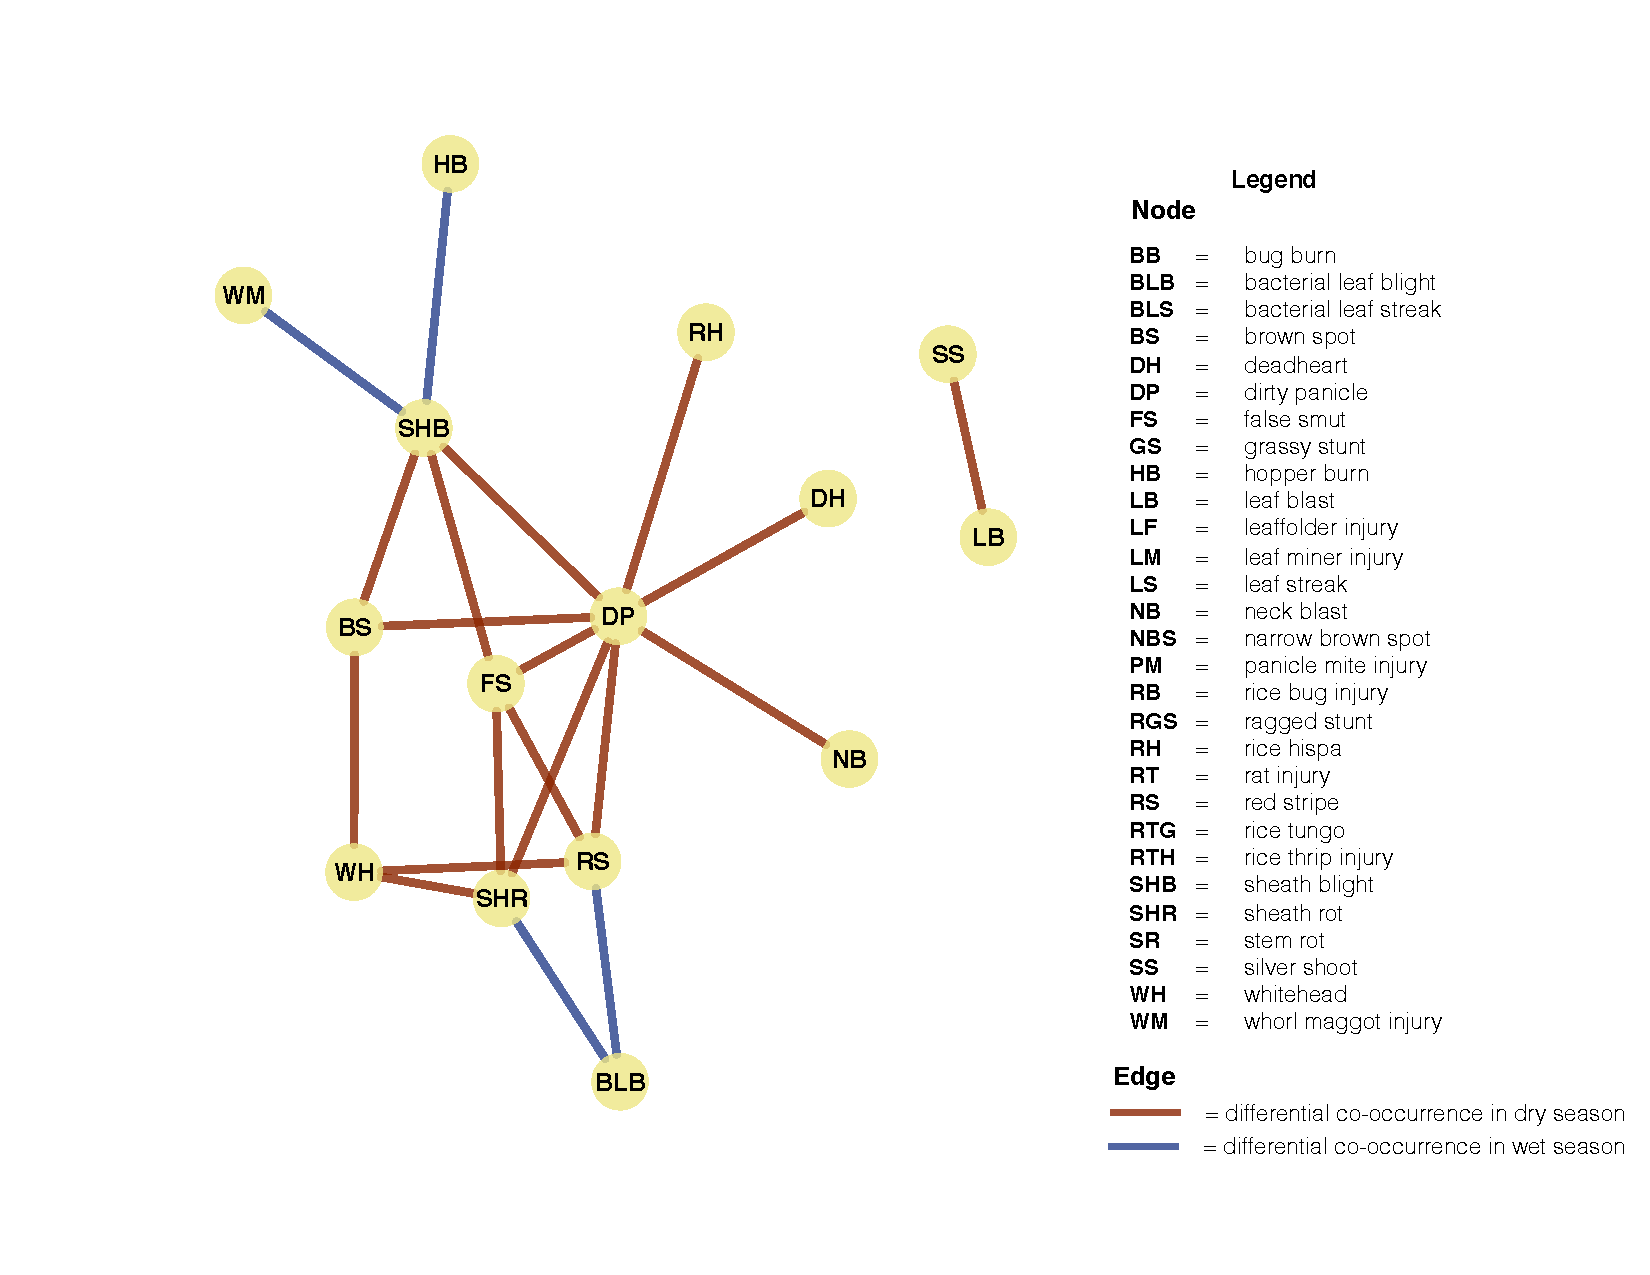
\includegraphics[width = 1\textwidth]{figures/difseasonCP.pdf}
\caption{Differential co-occurrence network of rice injuries in different seasons at Central Plain, Thailand}
\label{fig:difseasonCP}
\end{figure} 

\begin{figure}
\centering
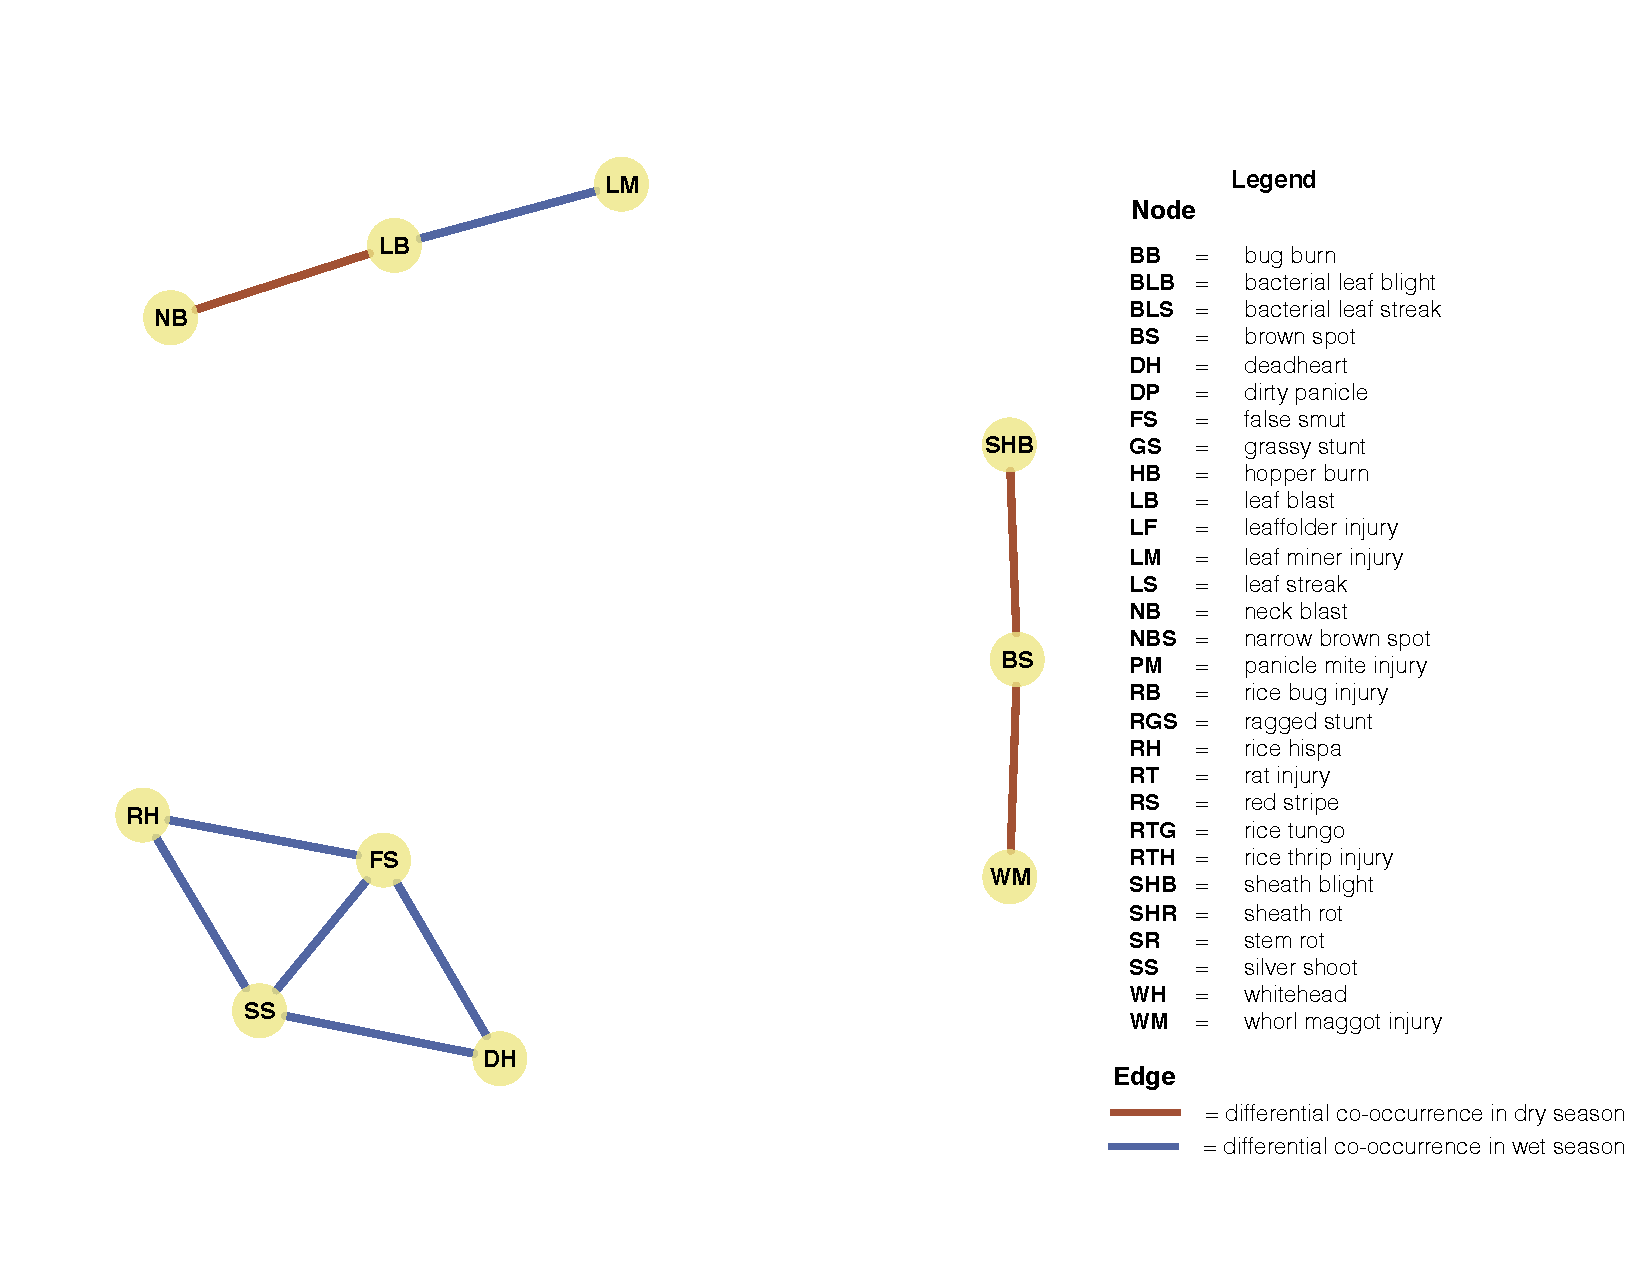
\includegraphics[width = 1\textwidth]{figures/difseasonOR.pdf}
\caption{Differential co-occurrence network of rice injuries in different seasons at Odisha, India }
\label{fig:difseasonOR}
\end{figure}


\begin{figure}
\centering
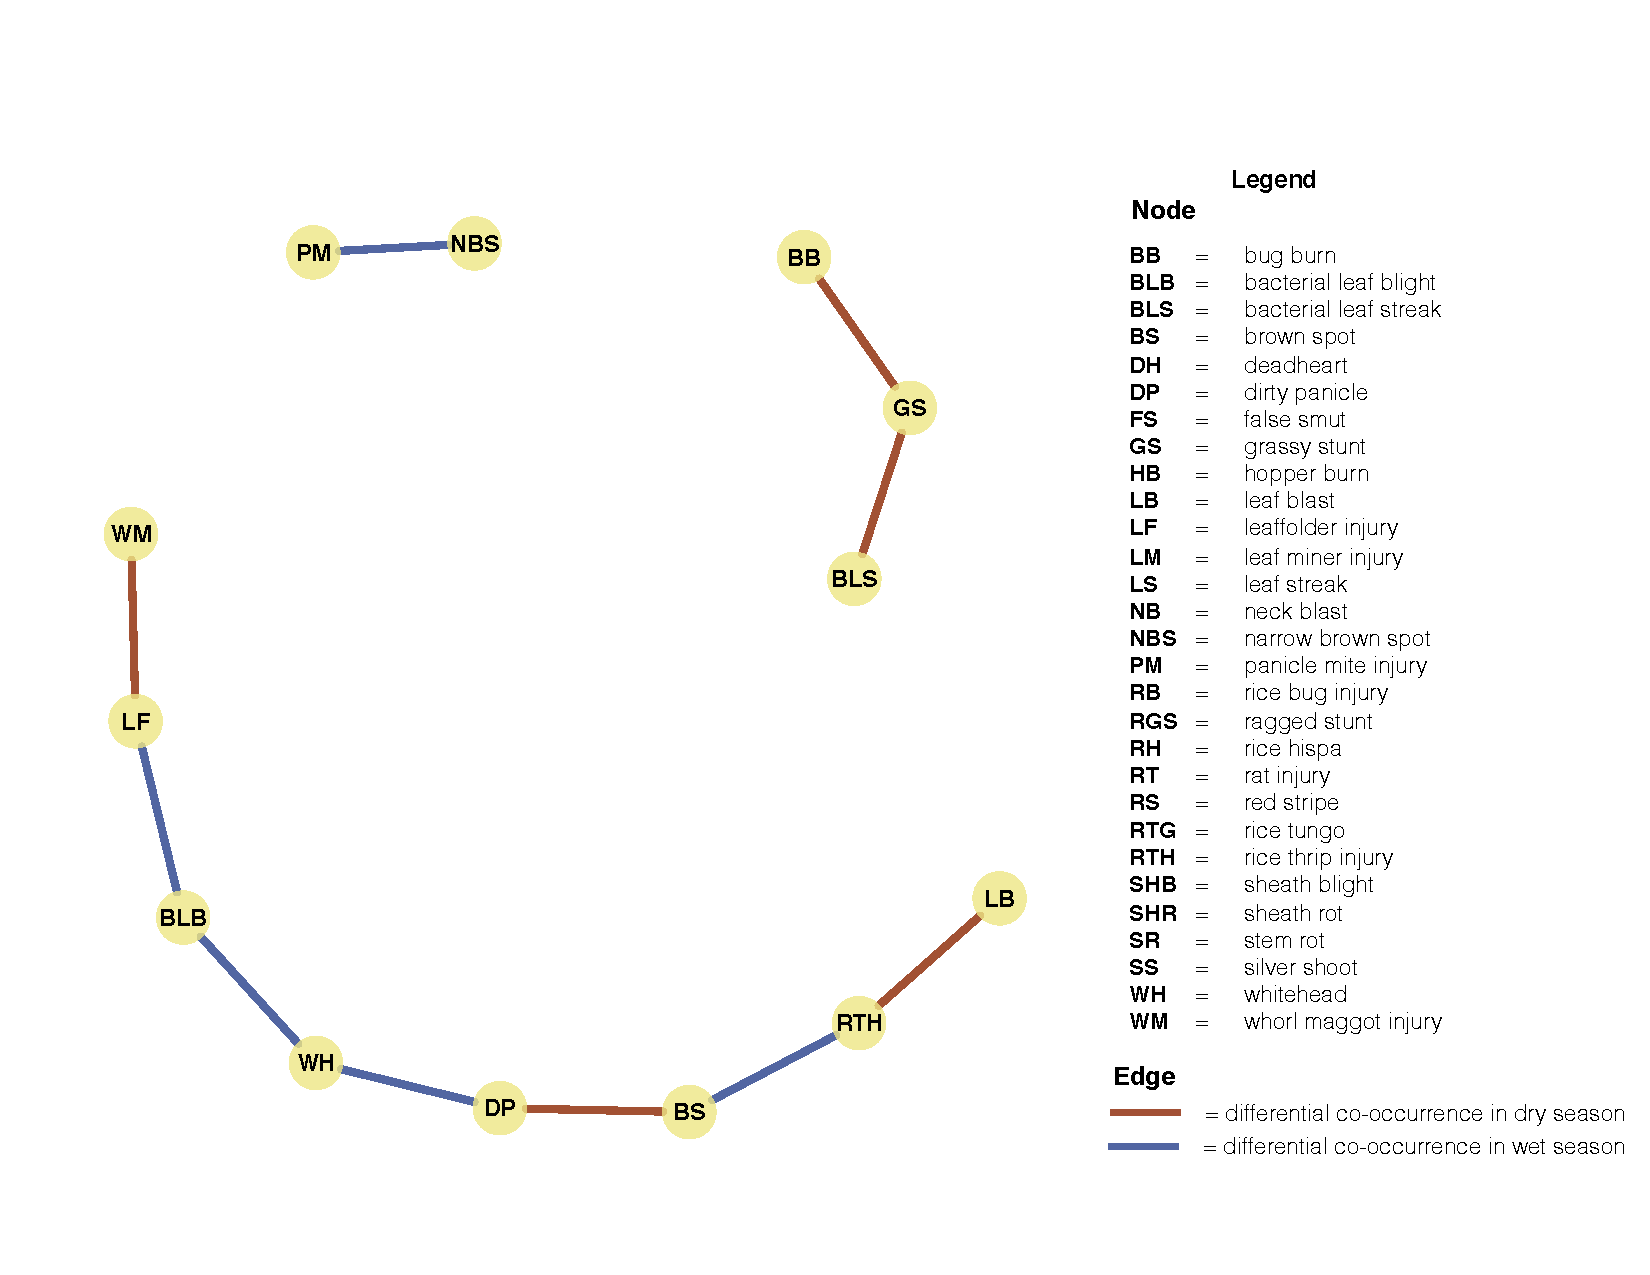
\includegraphics[width = 1\textwidth]{figures/difseasonRR.pdf}
\caption{Differential co-occurrence network of rice injuries in different seasons at Red River Delta, Vietnam}
\label{fig:difseasonRR}
\end{figure}


\begin{figure}
\centering
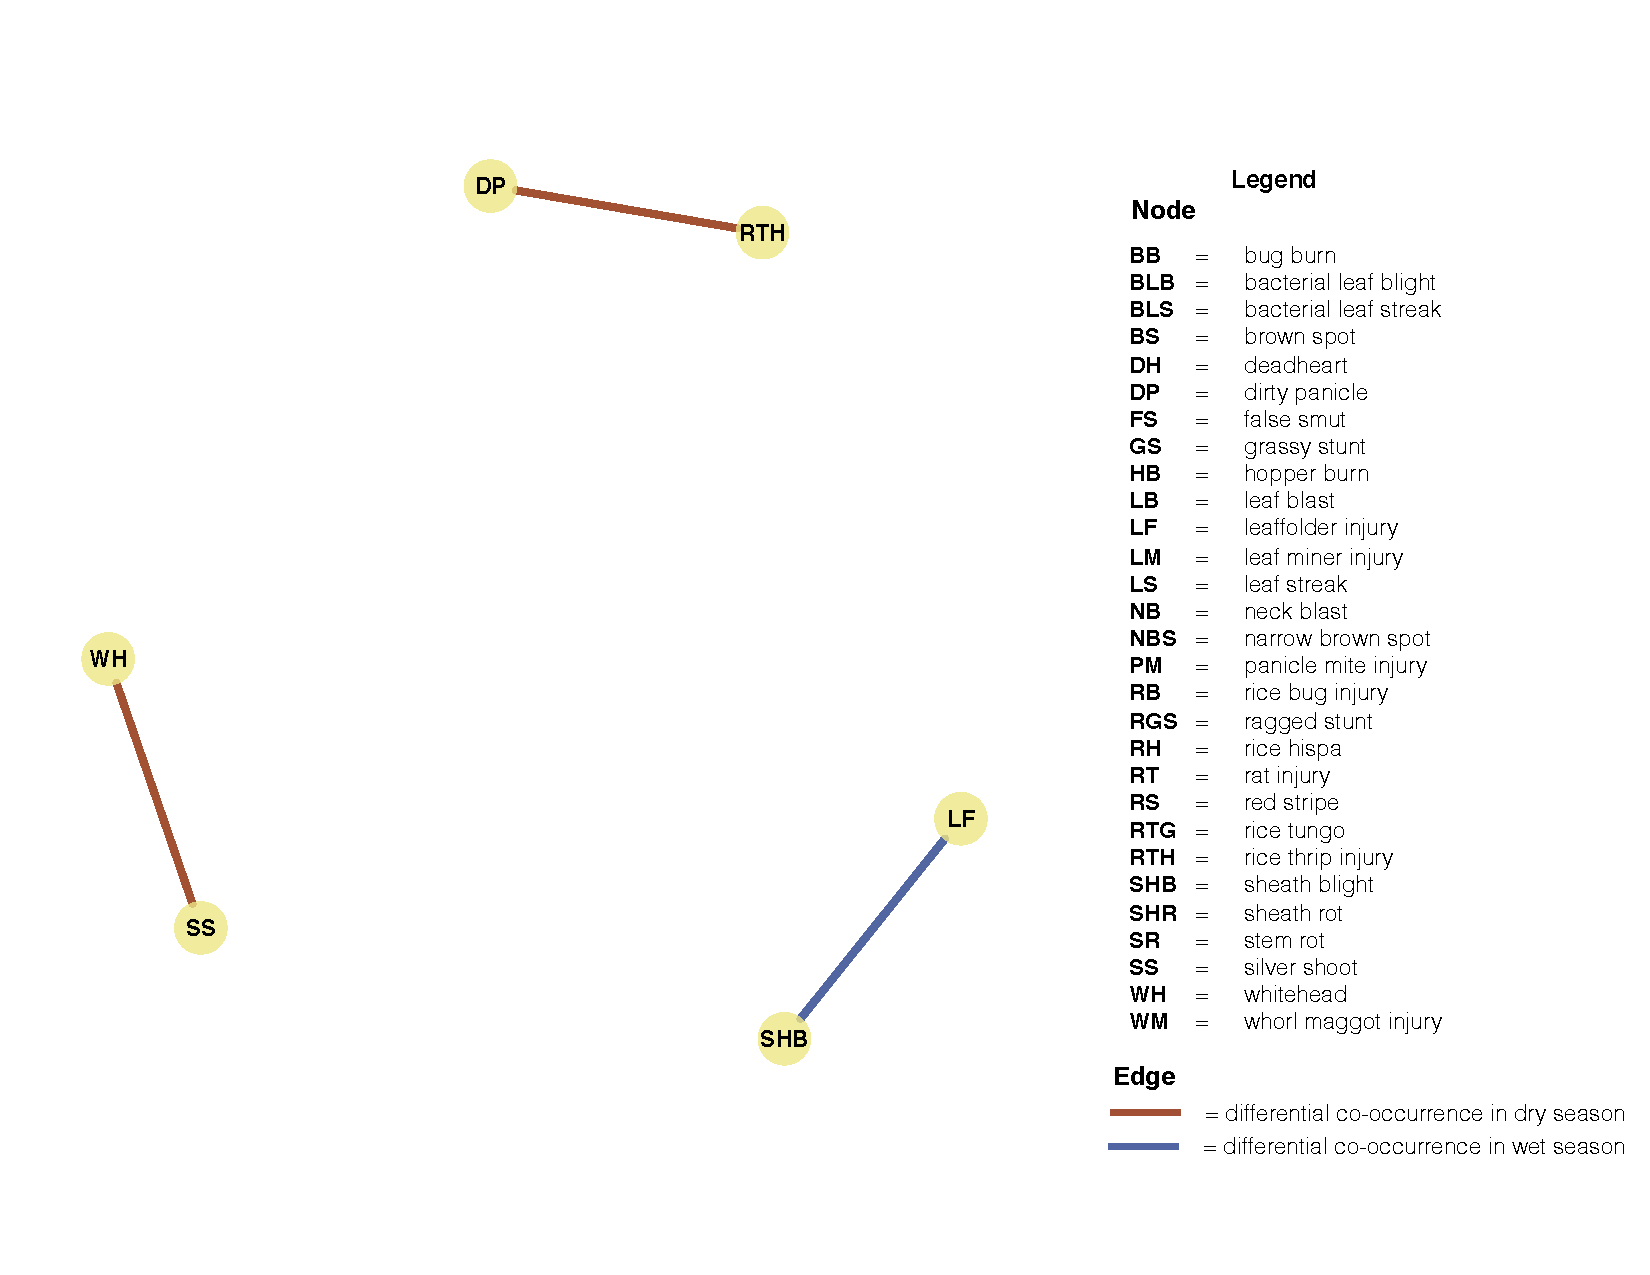
\includegraphics[width = 1\textwidth]{figures/difseasonTM.pdf}
\caption{Differential co-occurrence network of rice injuries in different seasons at Tamil Nadu, India}
\label{fig:difseasonTM}
\end{figure}


\begin{figure}
\centering
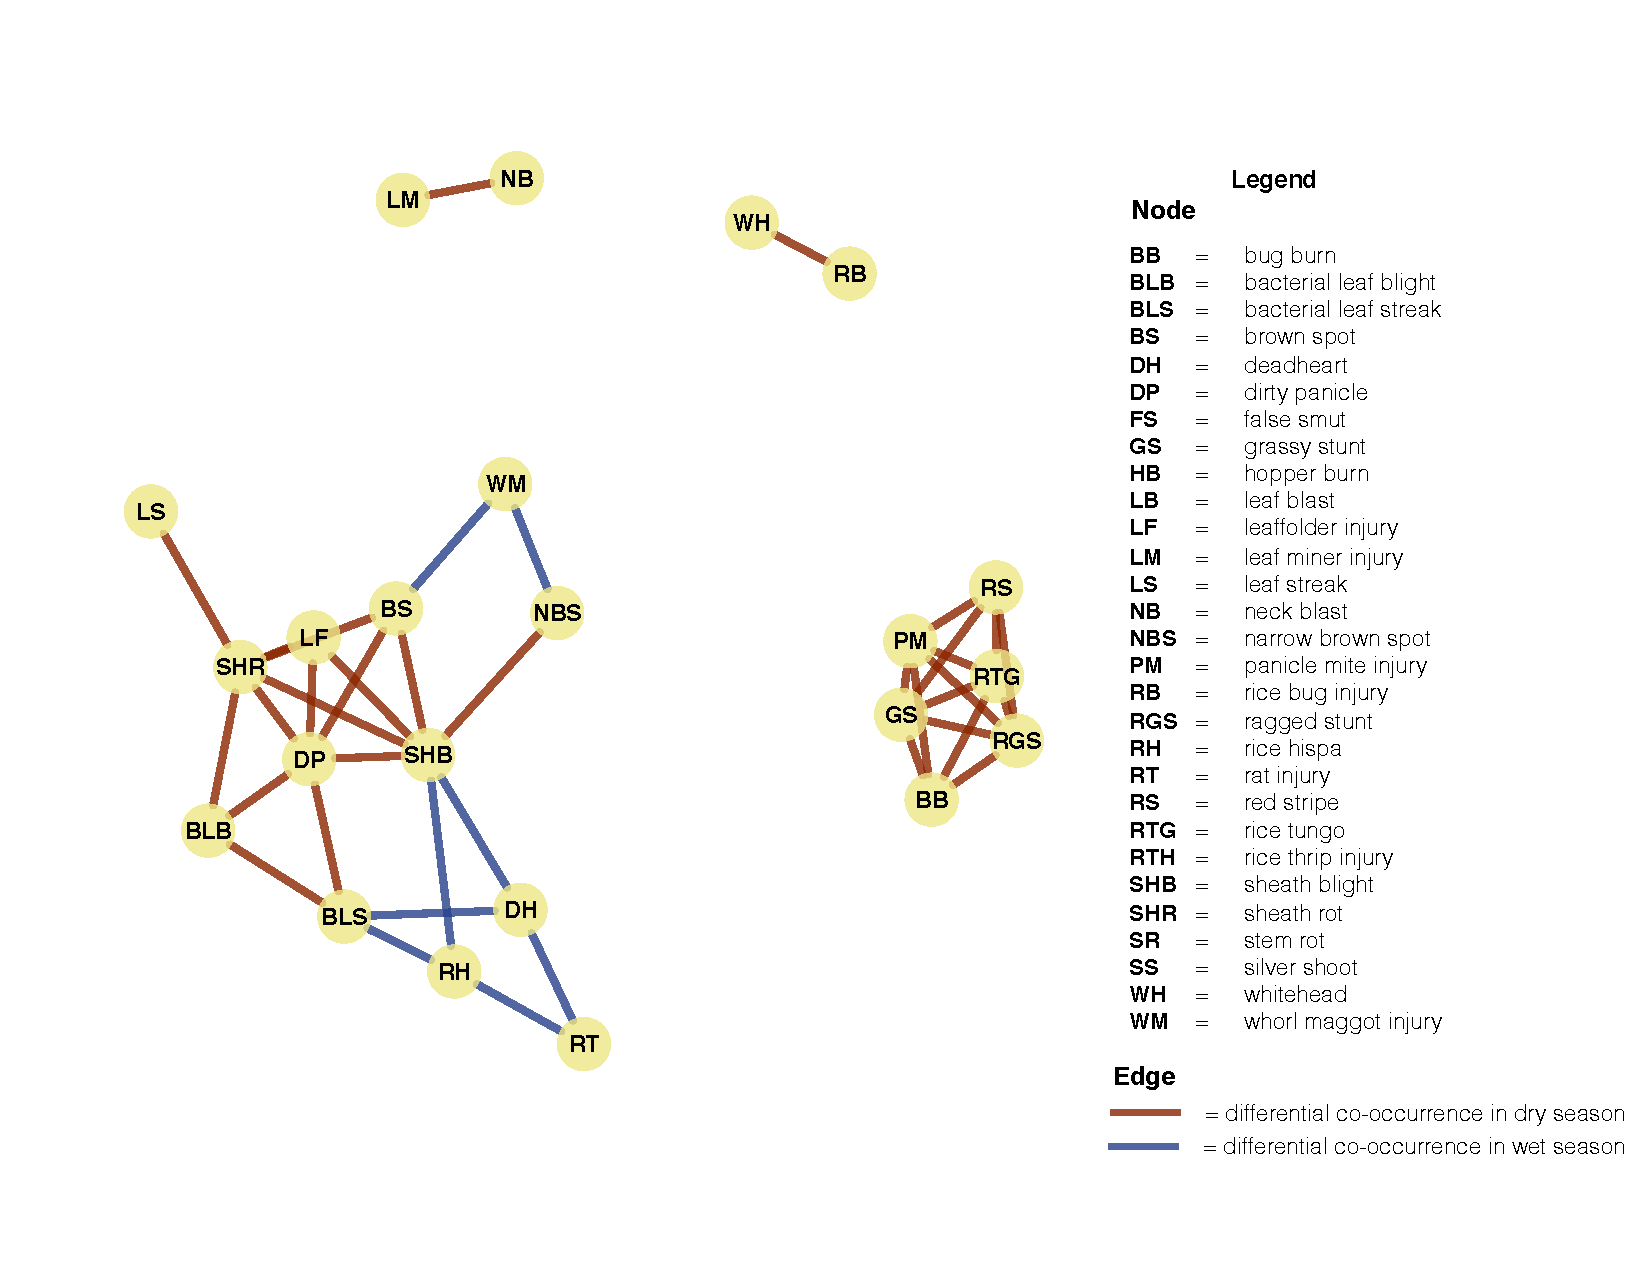
\includegraphics[width = 1\textwidth]{figures/difseasonWJ.pdf}
\caption{Differential co-occurrence network of rice injuries in different seasons at West Java, Indonesia}
\label{fig:difseasonWJ}
\end{figure}

%================================


\begin{figure}
    \centering
    \begin{subfigure}[b]{1\textwidth}
        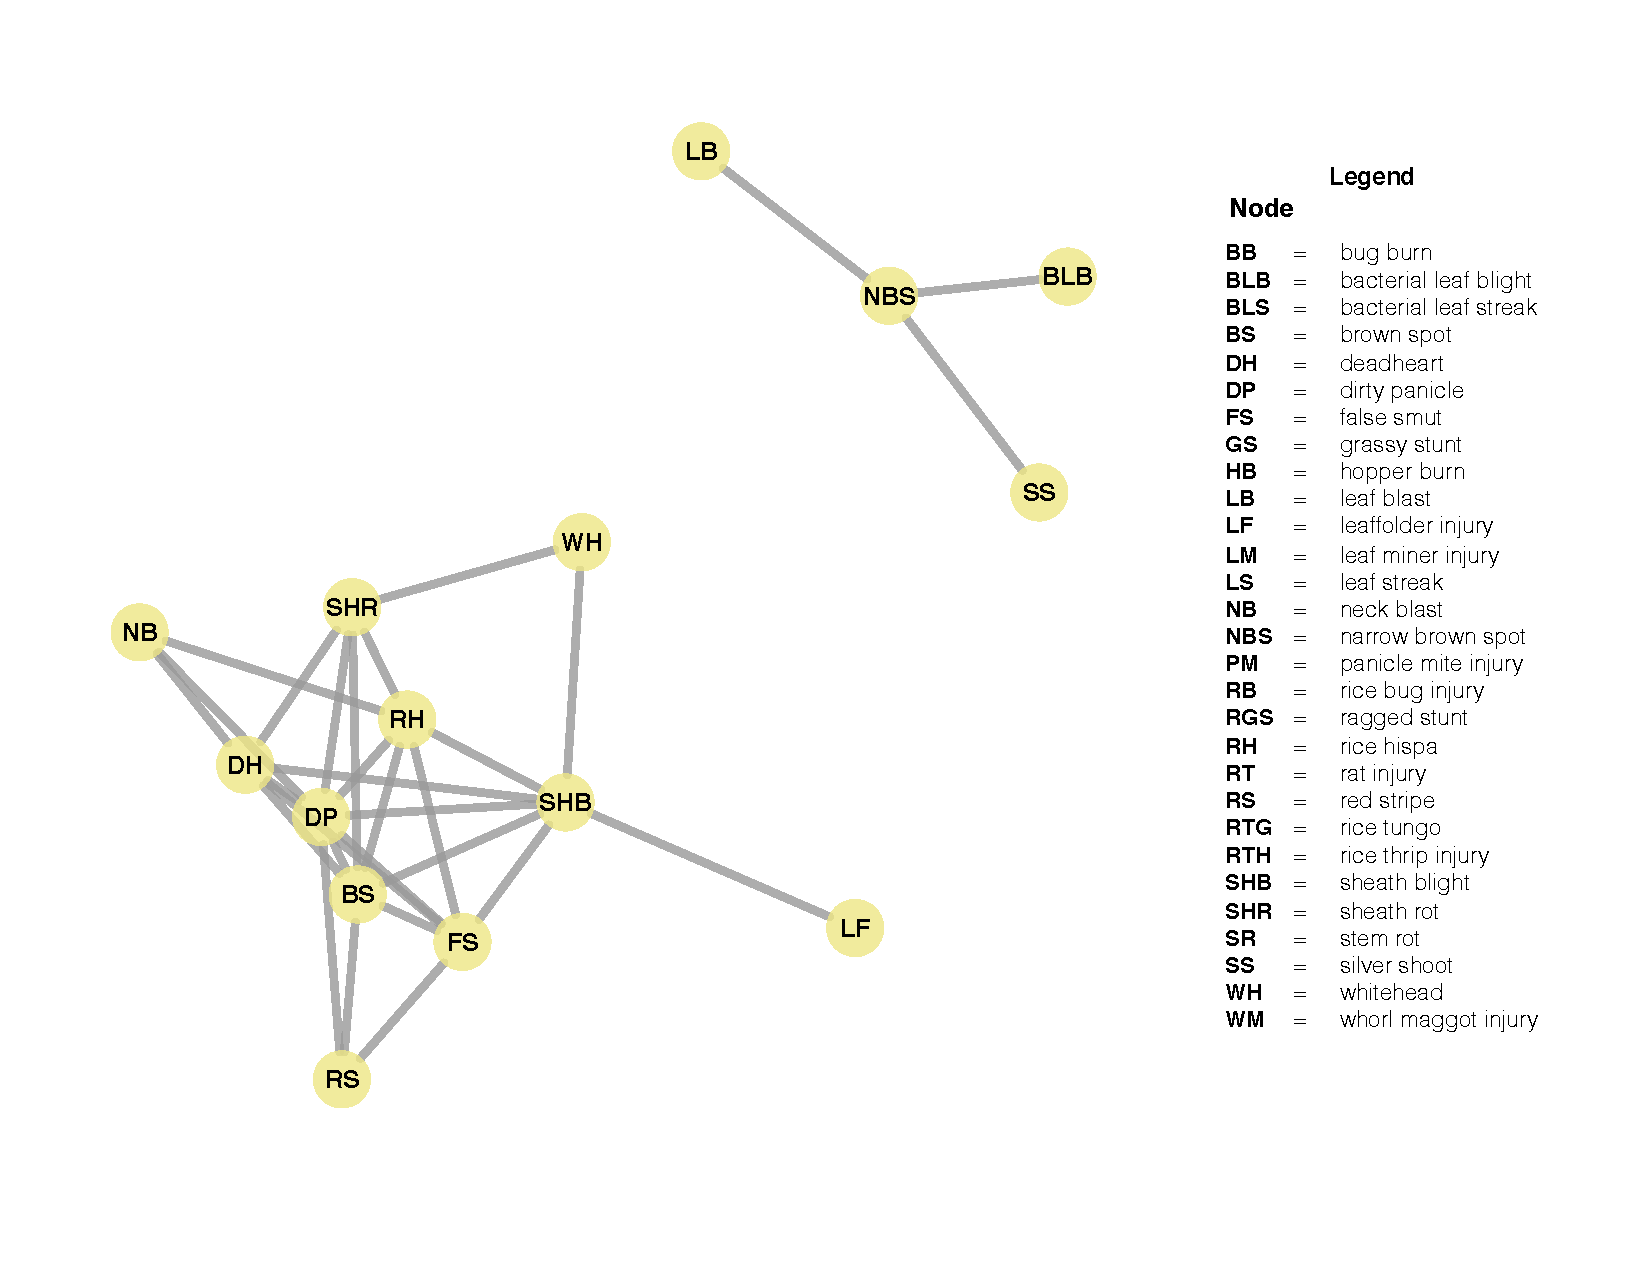
\includegraphics[width = 1\textwidth]{figures/difyieldCP.pdf}
        \caption{Differential co-occurrence network of rice injuries in different yield levels at Central Plain, Thailand. The layout of the network graph is based on the Fruchterman-Reingold algorithm, which places nodes with stronger or more connections closer to each other.}
        \label{fig:networkCP_ds}
    \end{subfigure}
    \begin{subfigure}[b]{1\textwidth}
        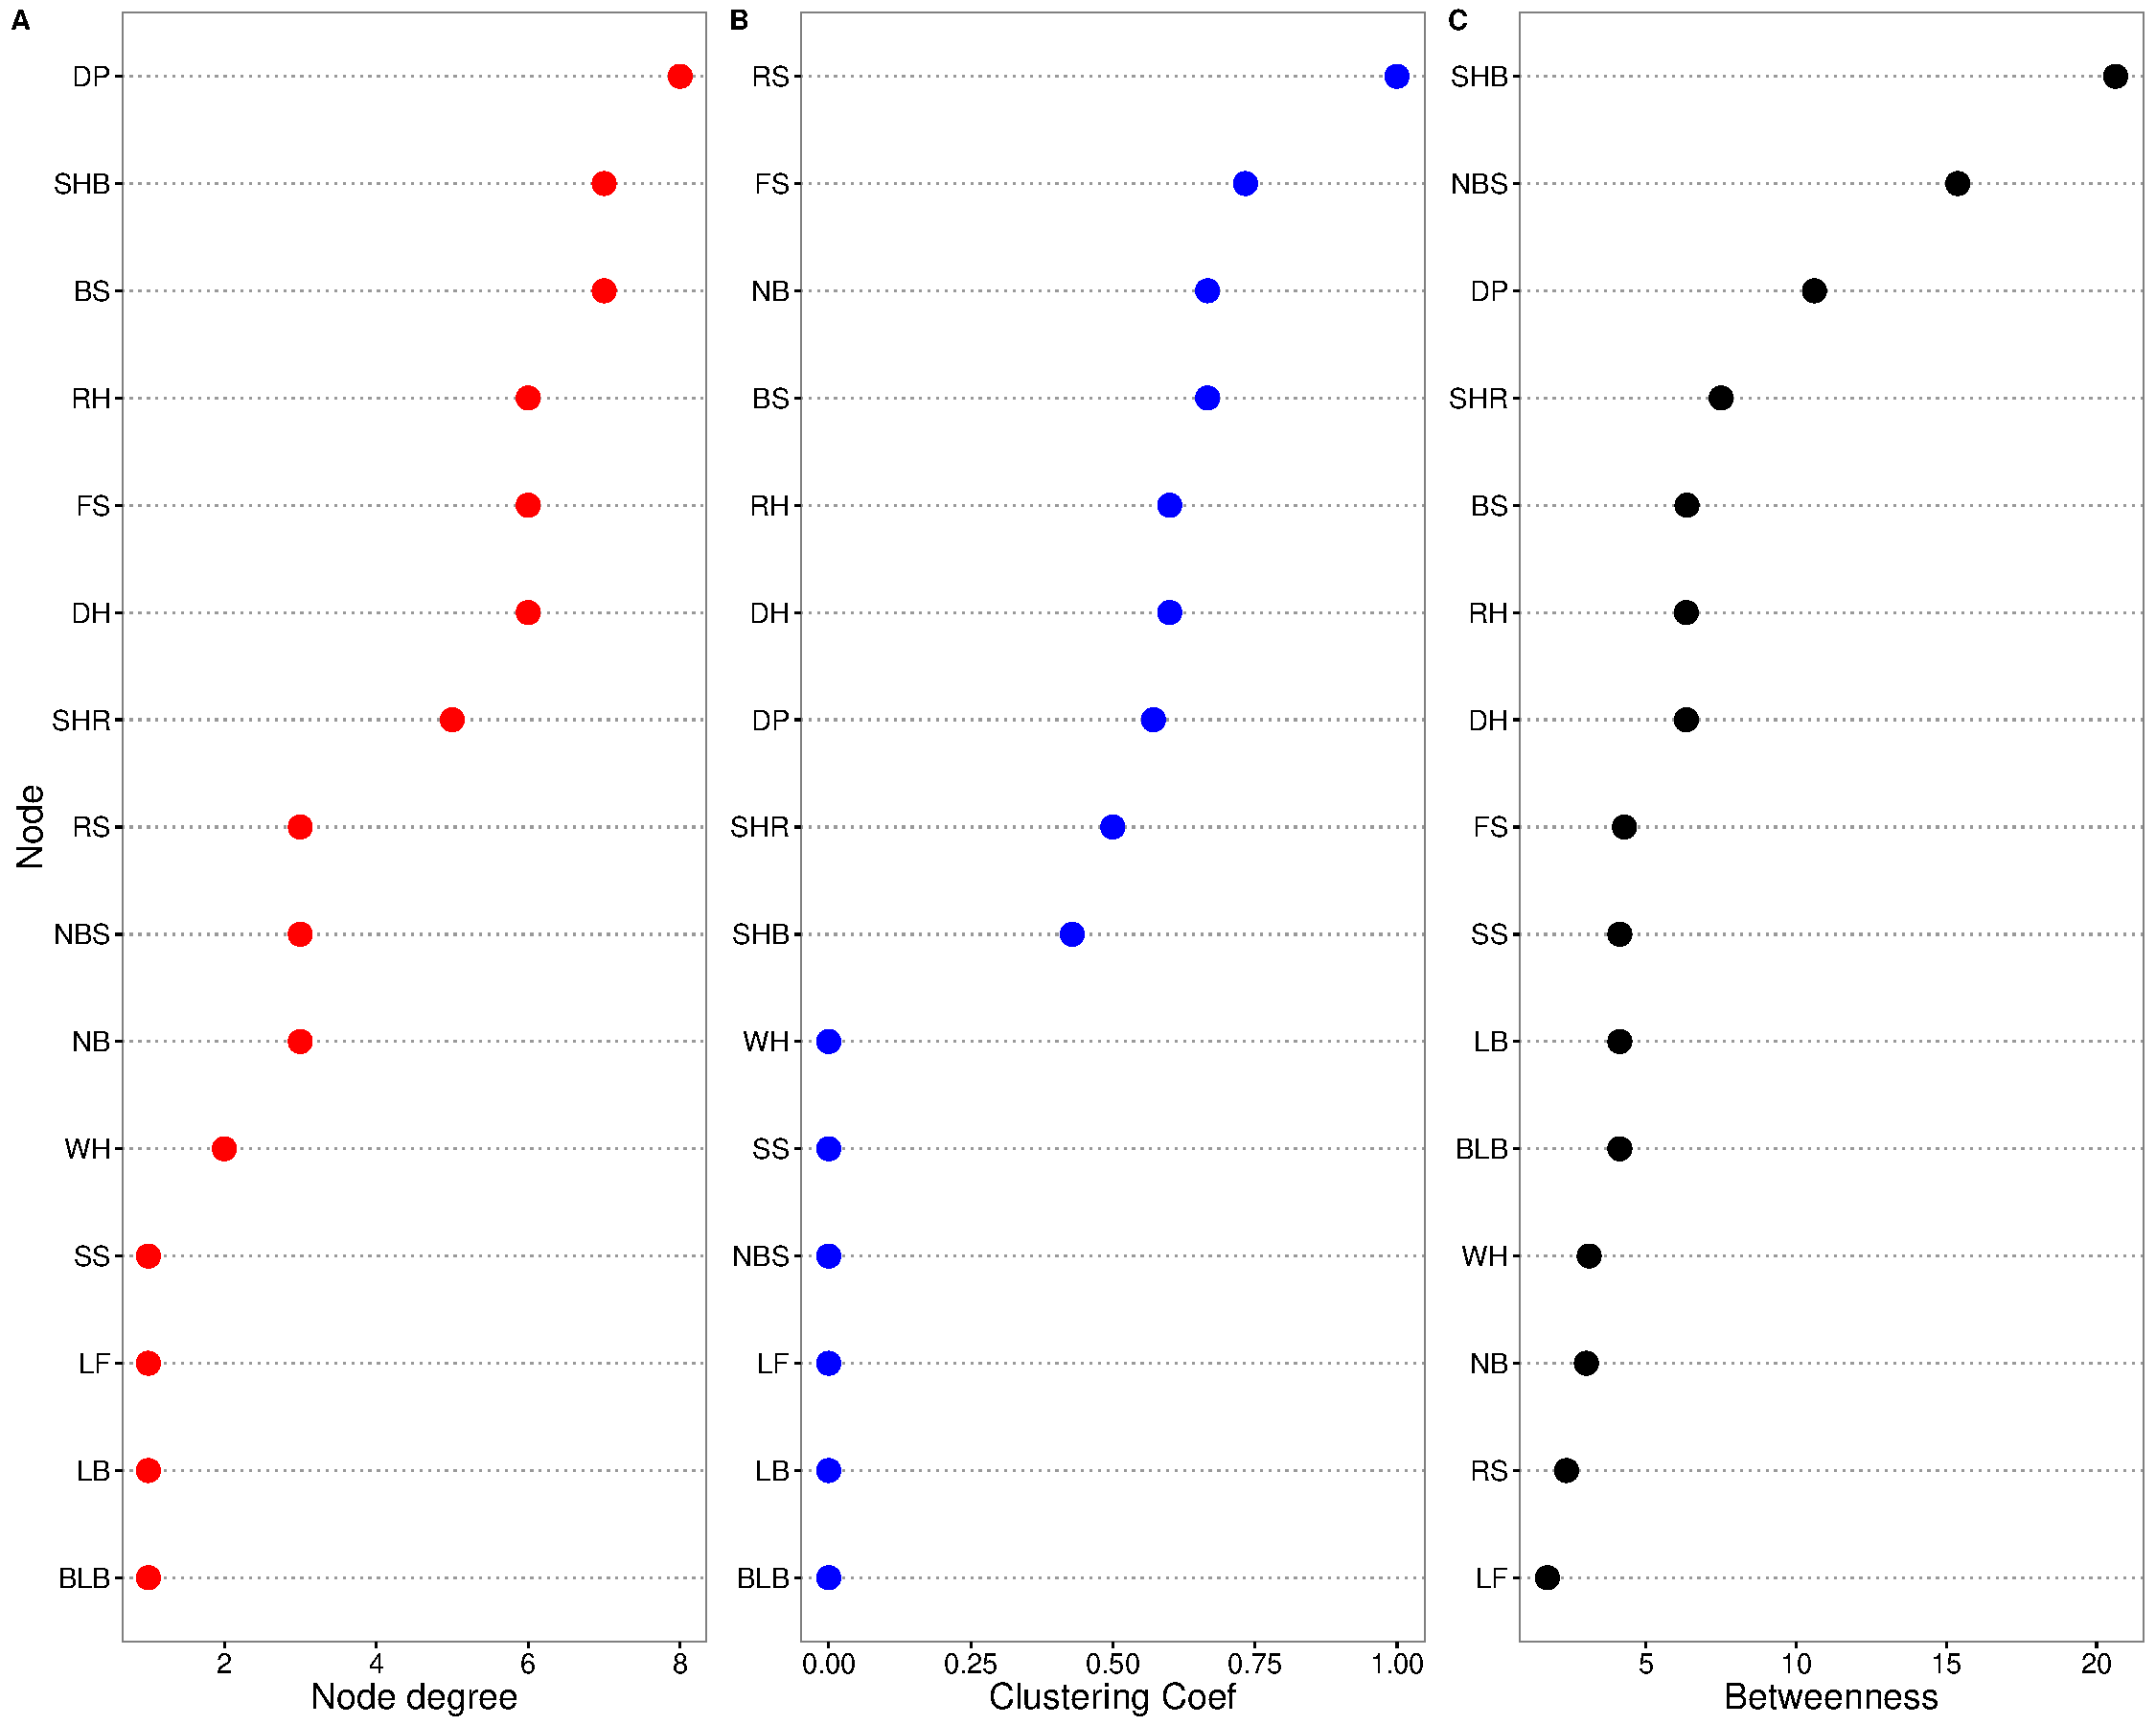
\includegraphics[width = 1\textwidth]{figures/yield_dif_nodepropCentral_Plain.pdf}
        \caption{Three centrality measures of the nodes in co-occurrence network of rice injuries in dry season at Central Plain. A: node degree, B:clustering coefficient, and C:Betweenness.}
        \label{fig:nodepropCP_ds}
    \end{subfigure}
    \caption{Rice injuries in dry season in Central Plain, Thailand}
    \label{fig:CP_ds}
\end{figure}
 
\begin{figure}
    \centering
    \begin{subfigure}[b]{1\textwidth}
        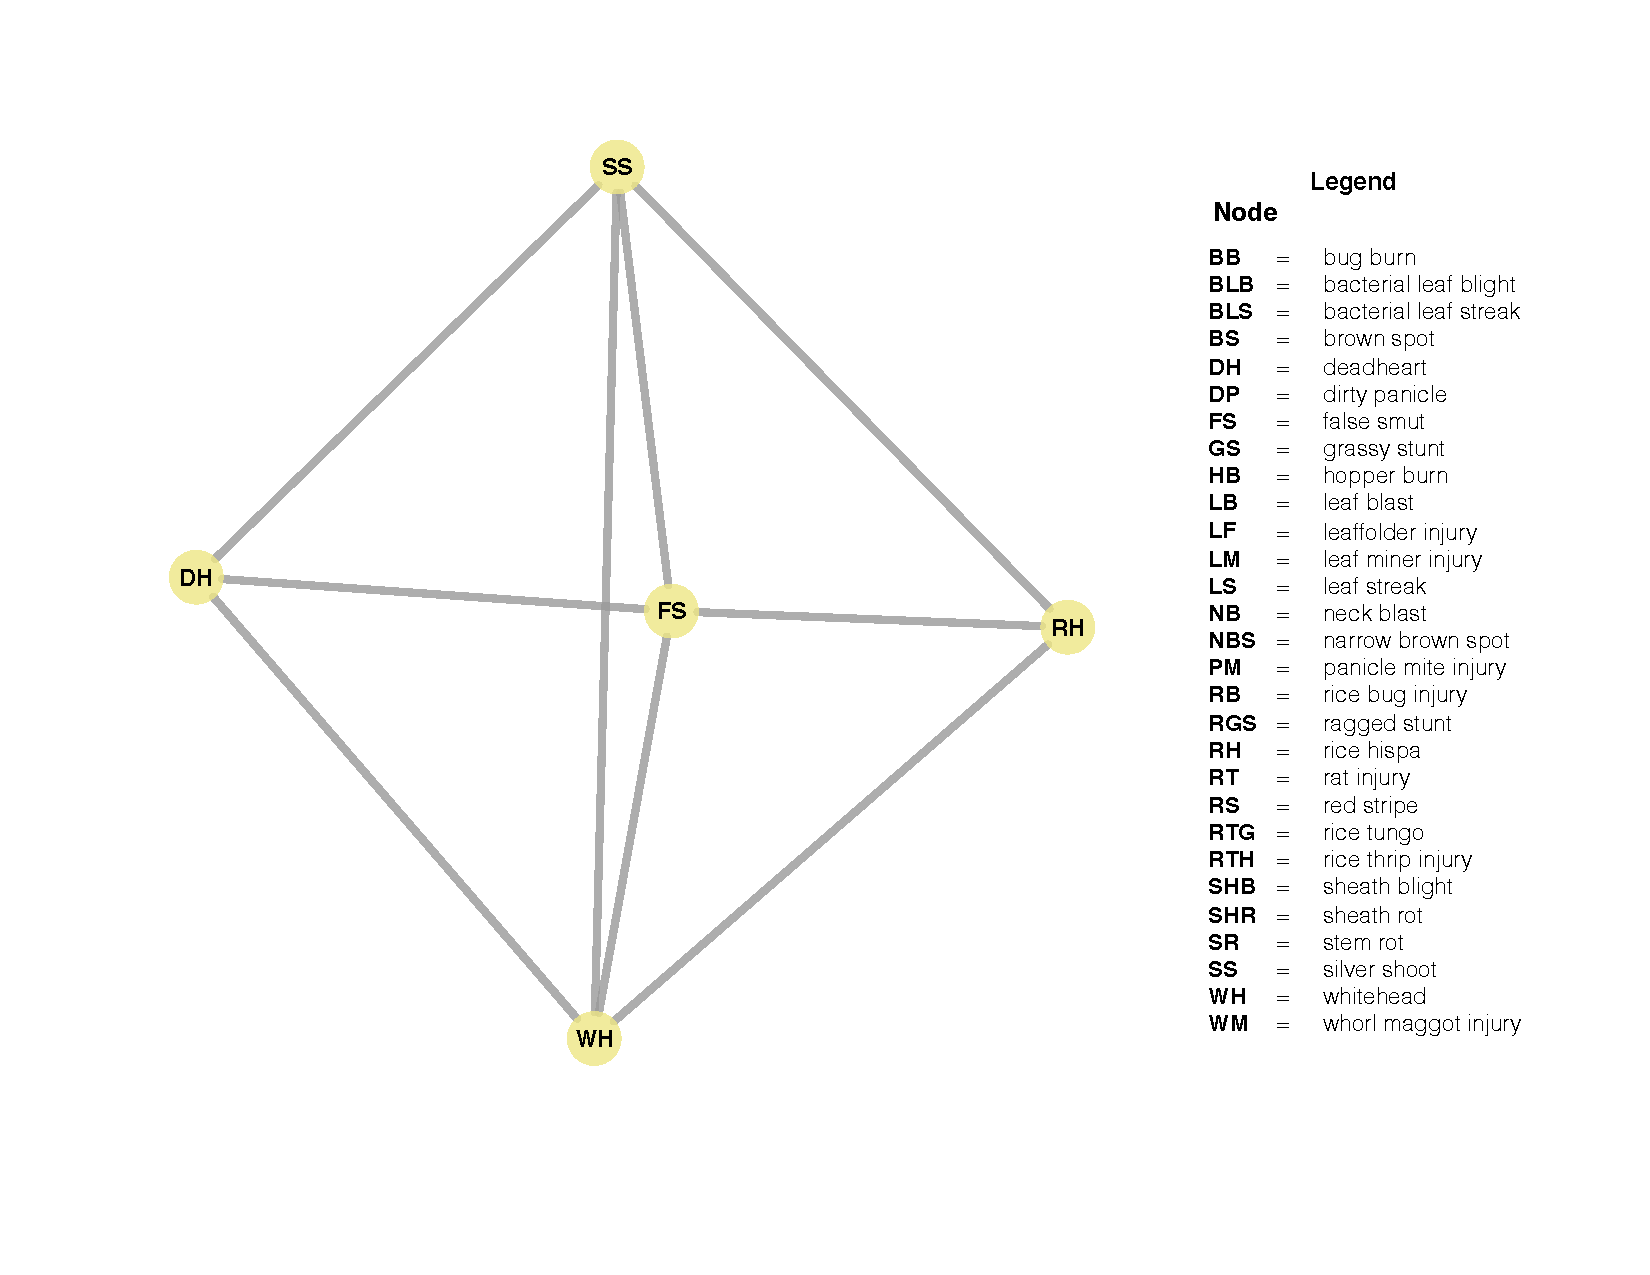
\includegraphics[width = 1\textwidth]{figures/difyieldOD.pdf}
        \caption{Differential co-occurrence network of rice injuries in different yield levels at Central Plain, Thailand. The layout of the network graph is based on the Fruchterman-Reingold algorithm, which places nodes with stronger or more connections closer to each other.}
        \label{fig:networkCP_ds}
    \end{subfigure}
    \begin{subfigure}[b]{1\textwidth}
        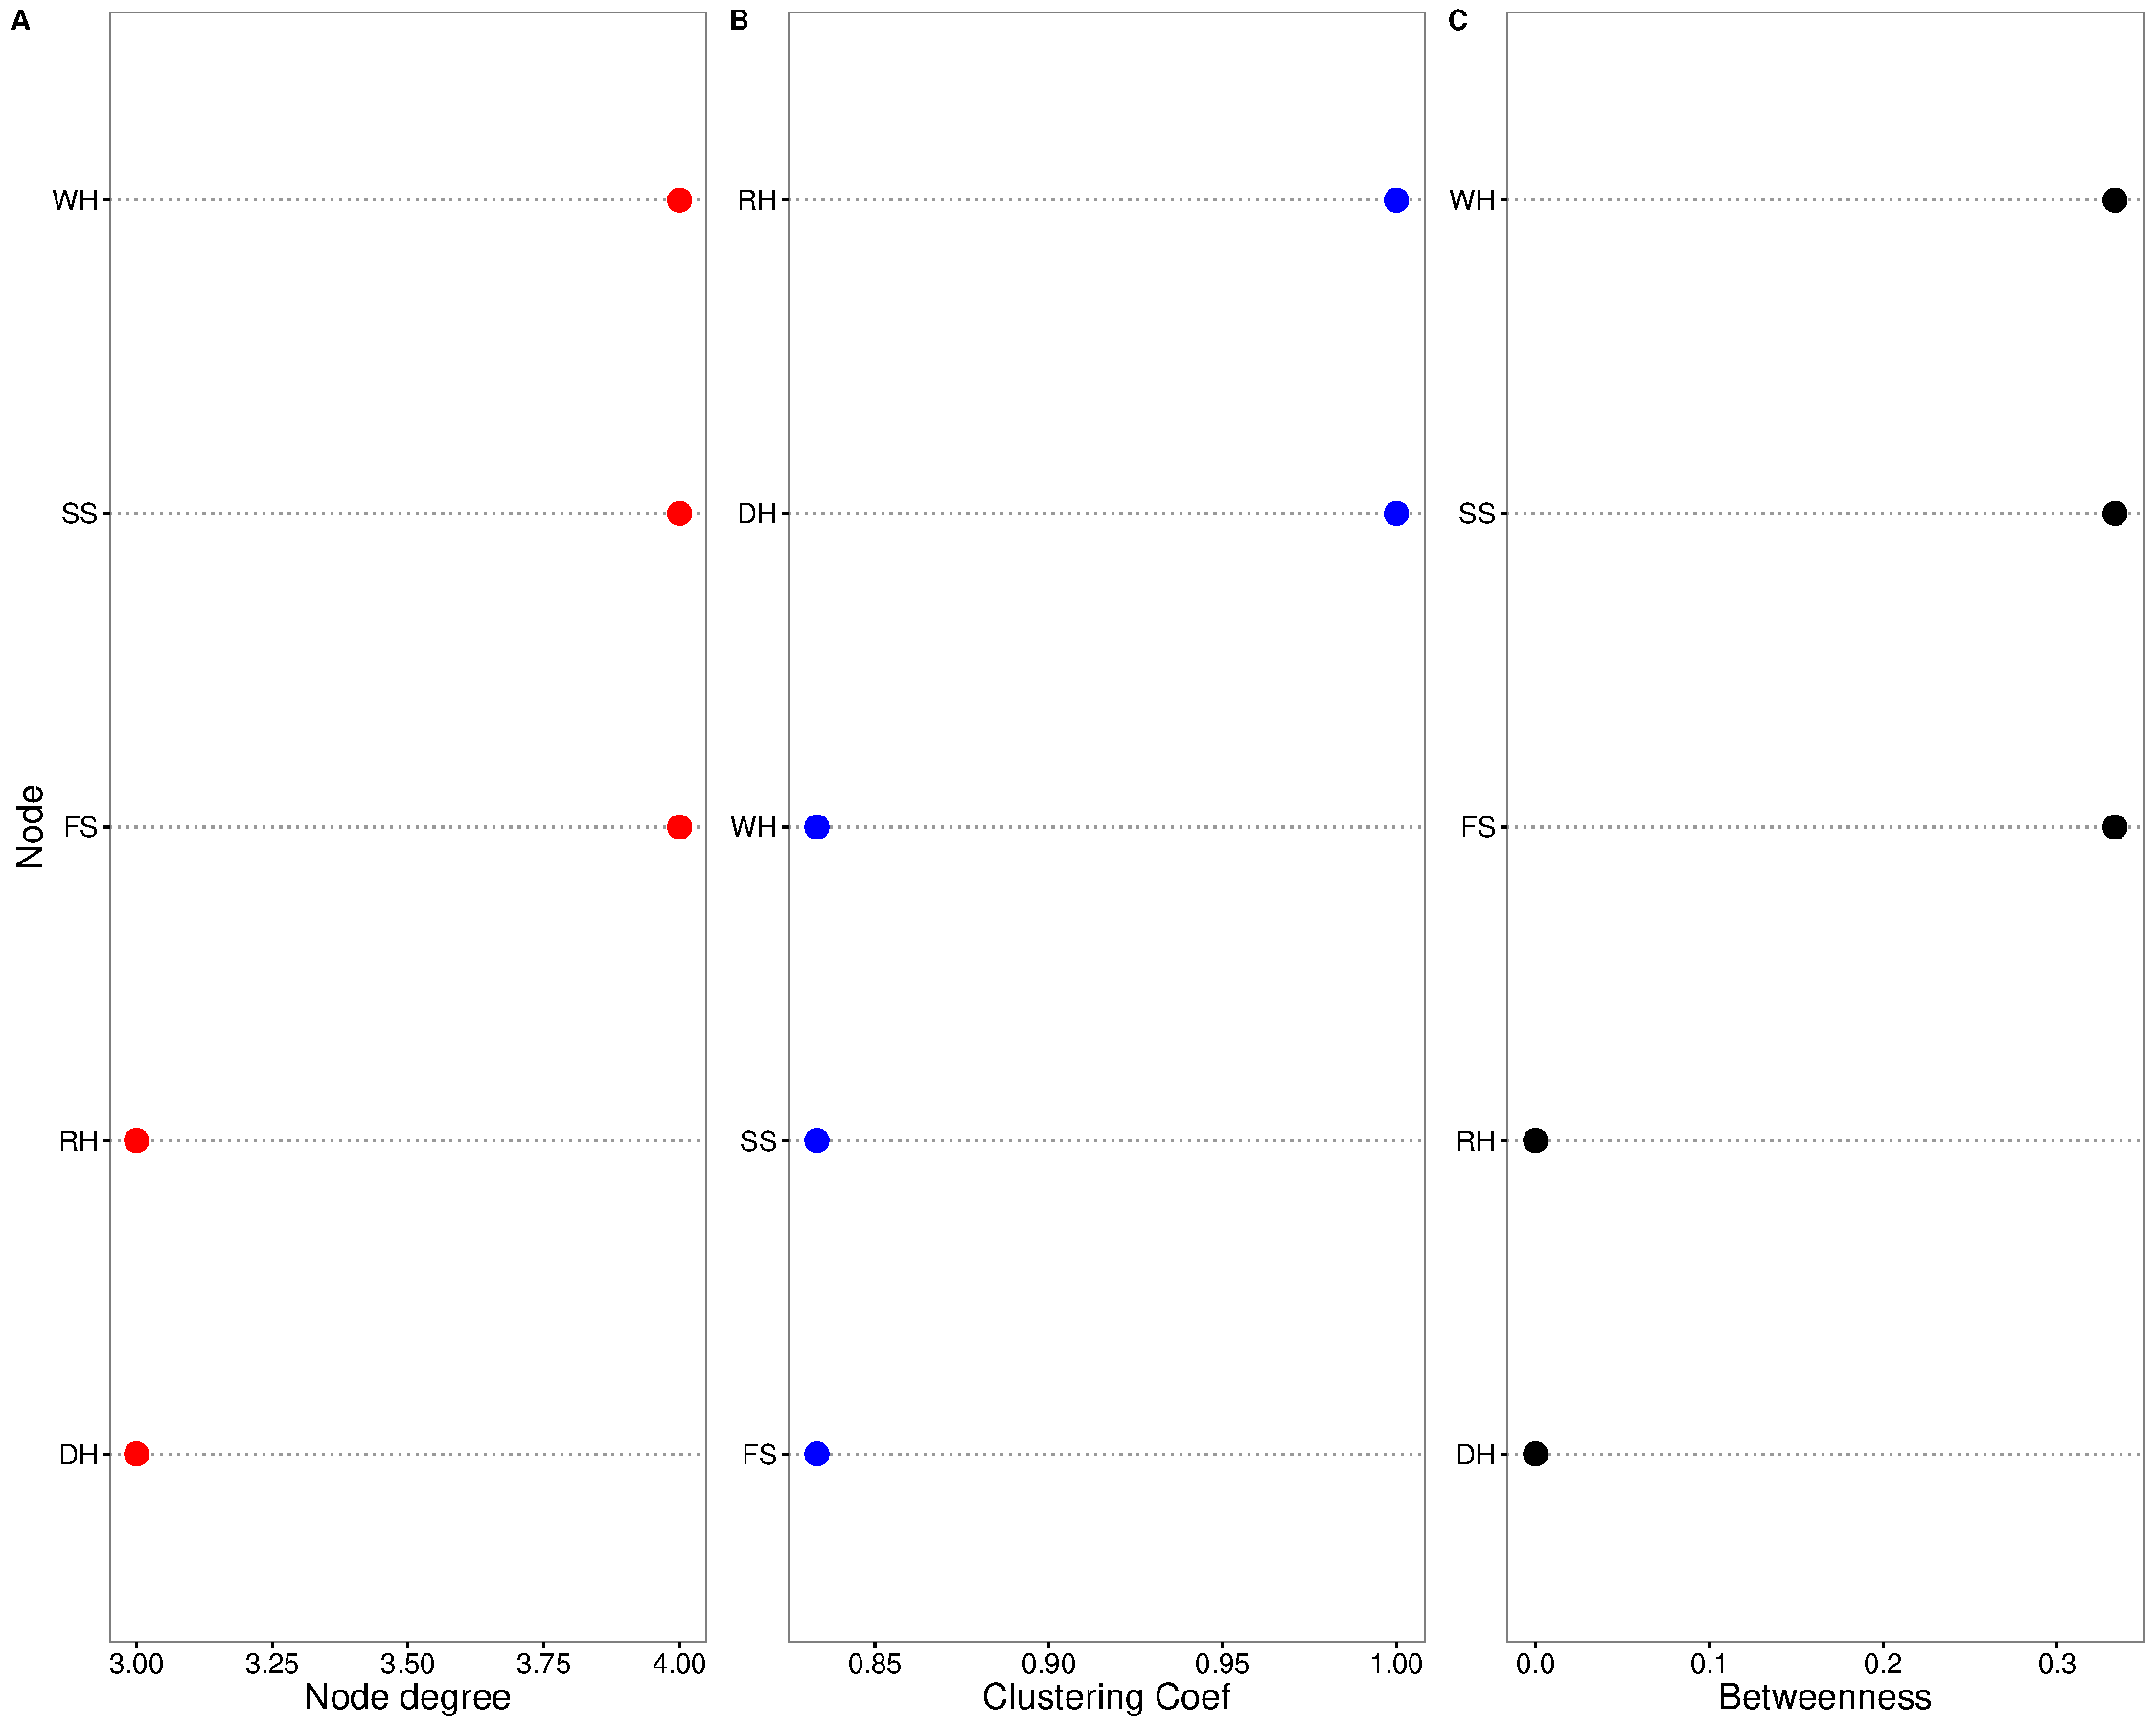
\includegraphics[width = 1\textwidth]{figures/yield_dif_nodepropOdisha.pdf}
        \caption{Three centrality measures of the nodes in co-occurrence network of rice injuries in dry season at Central Plain. A: node degree, B:clustering coefficient, and C:Betweenness.}
        \label{fig:nodepropCP_ds}
    \end{subfigure}
    \caption{Rice injuries in dry season in Central Plain, Thailand}
    \label{fig:CP_ds}
\end{figure}
 
 \begin{figure}
    \centering
    \begin{subfigure}[b]{1\textwidth}
        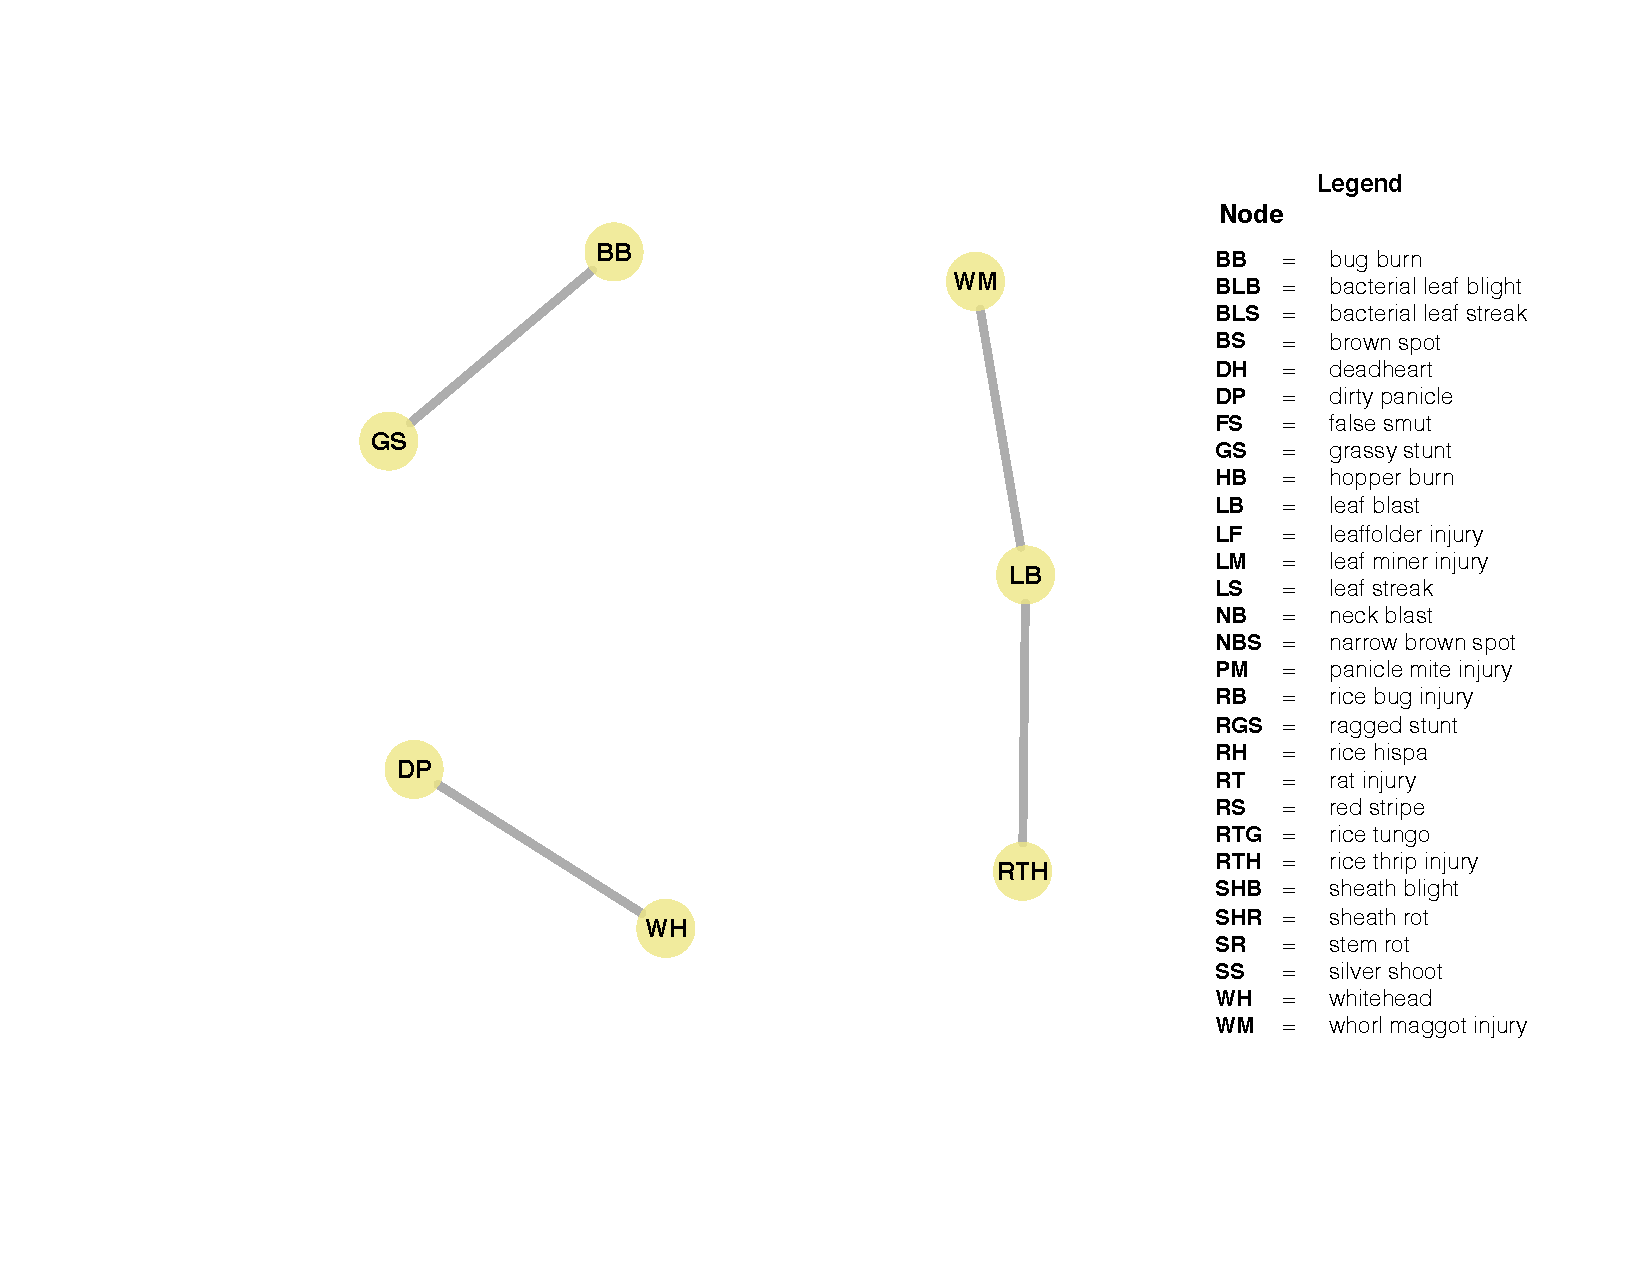
\includegraphics[width = 1\textwidth]{figures/difyieldRR.pdf}
        \caption{Differential co-occurrence network of rice injuries in different yield levels at Central Plain, Thailand. The layout of the network graph is based on the Fruchterman-Reingold algorithm, which places nodes with stronger or more connections closer to each other.}
        \label{fig:networkCP_ds}
    \end{subfigure}
    \begin{subfigure}[b]{1\textwidth}
        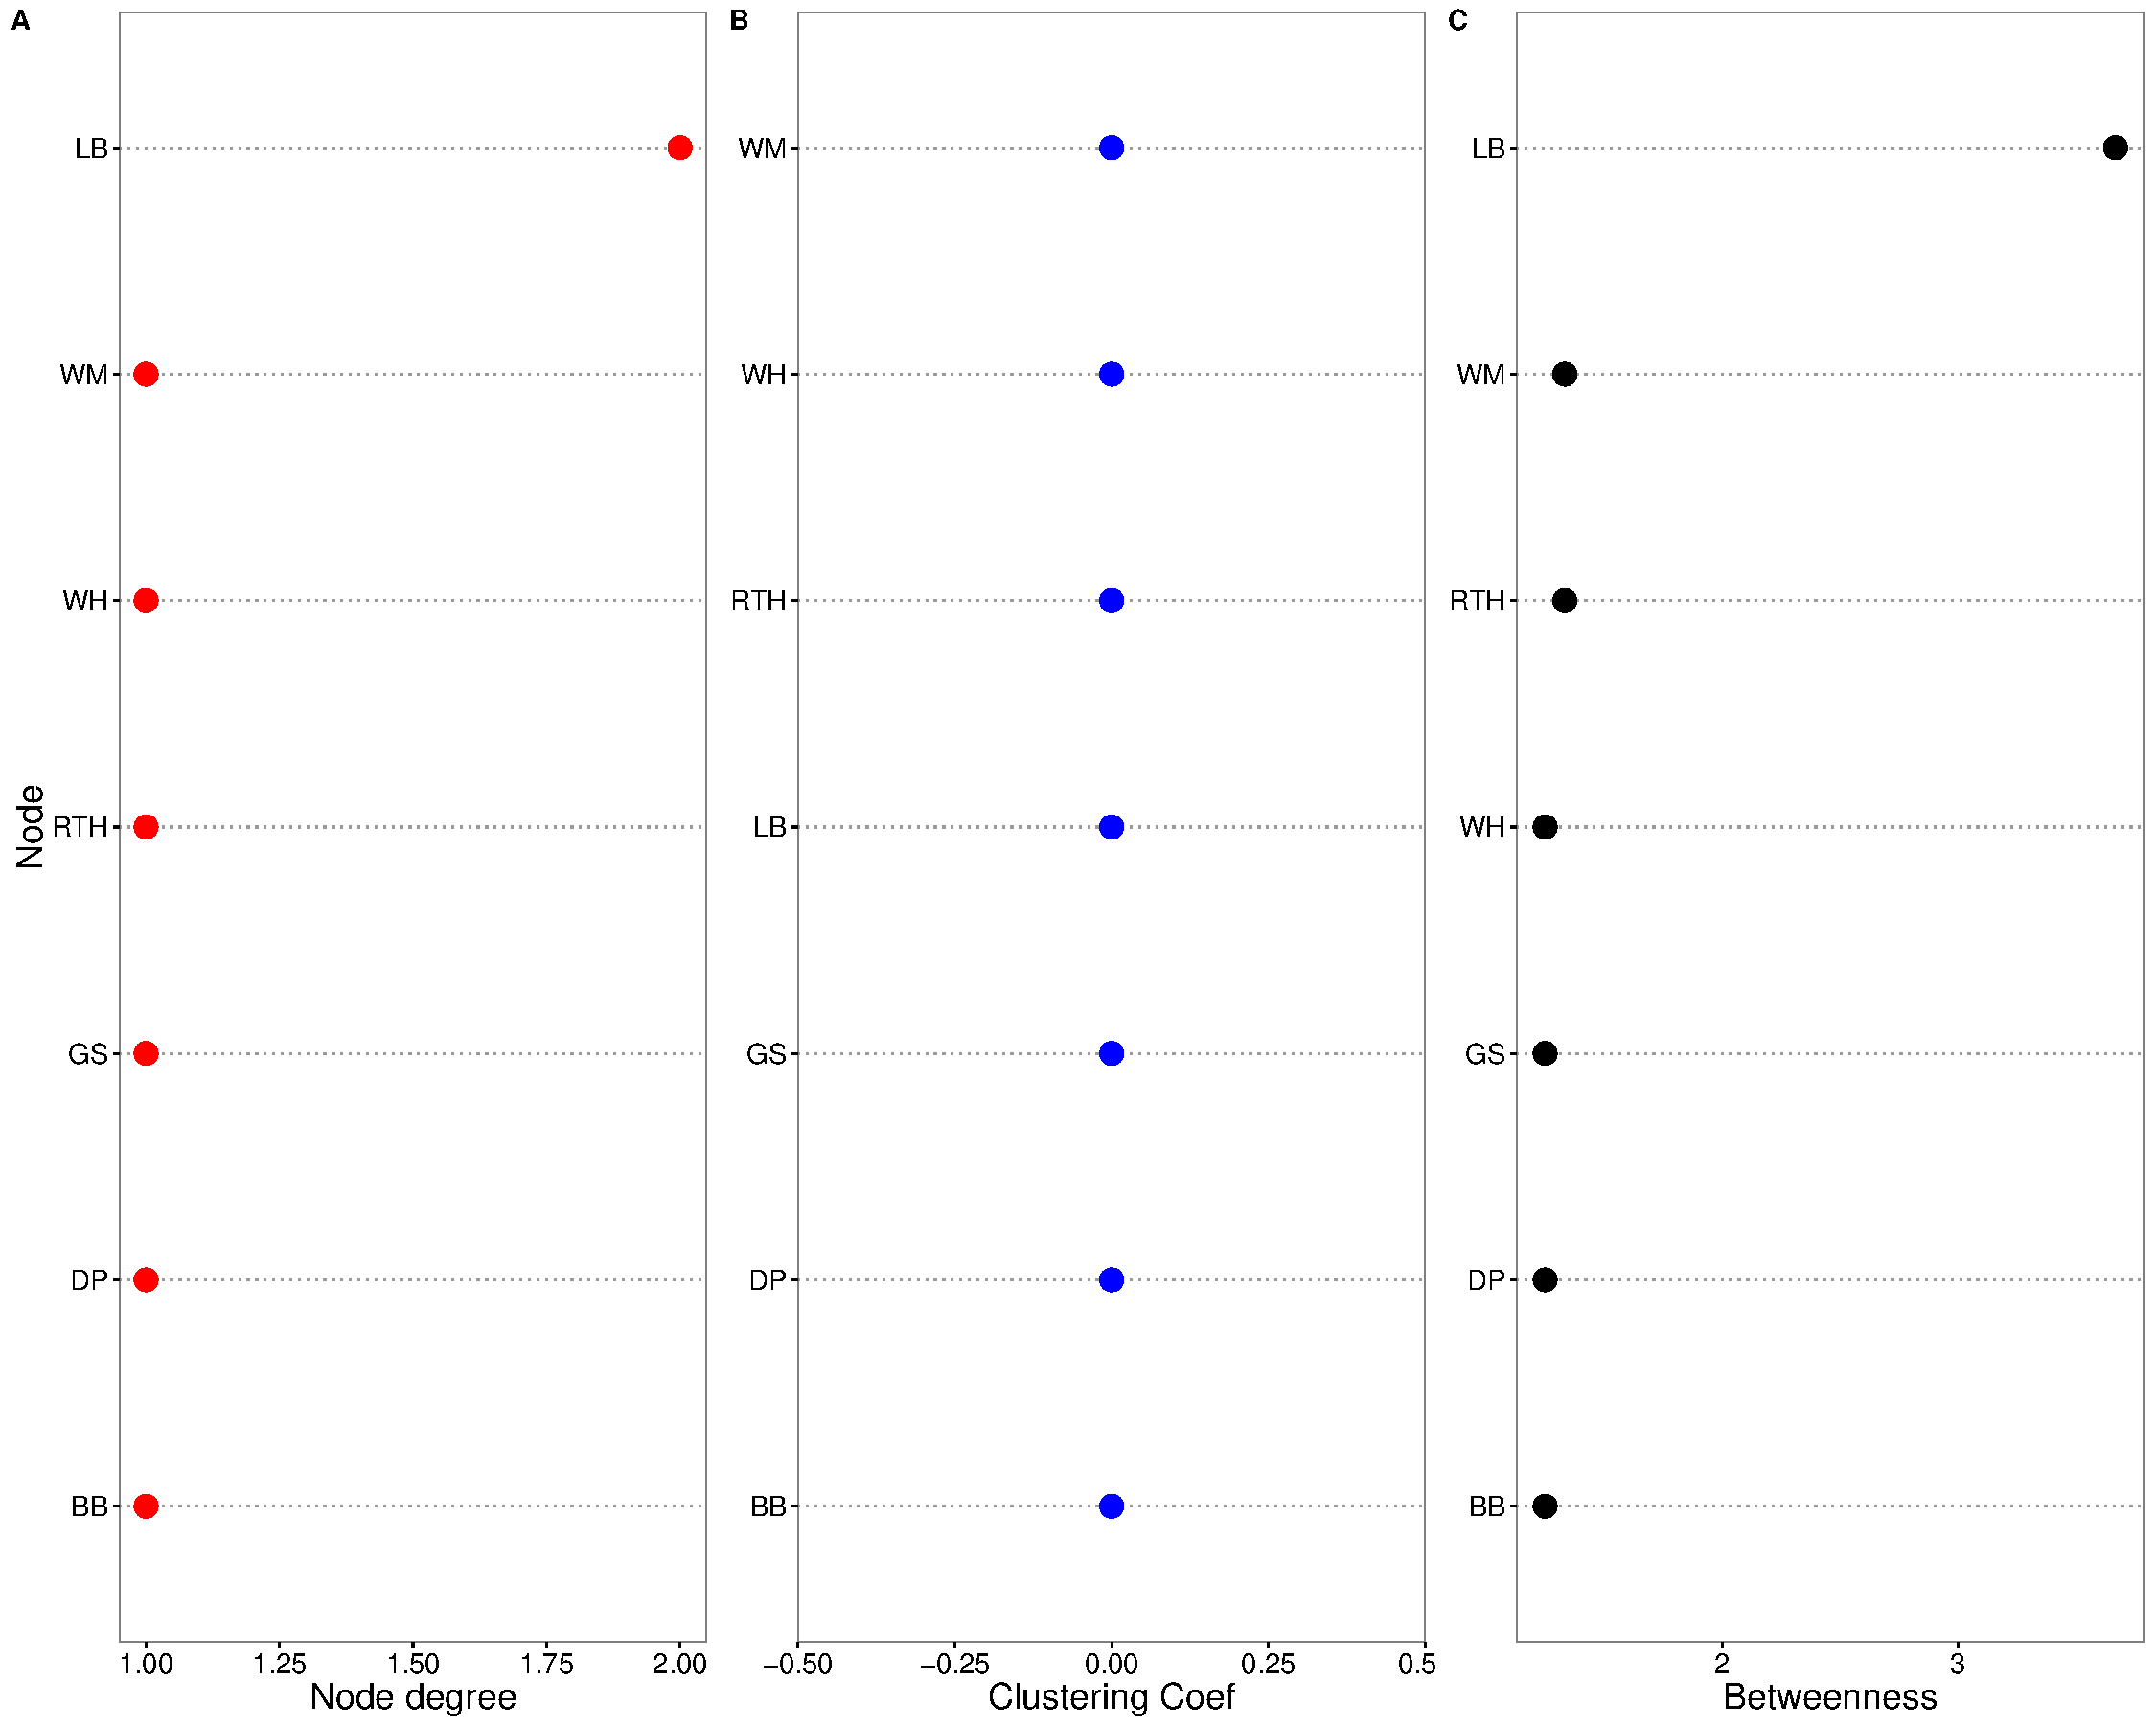
\includegraphics[width = 1\textwidth]{figures/yield_dif_nodepropRed_River_Delta.pdf}
        \caption{Three centrality measures of the nodes in co-occurrence network of rice injuries in dry season at Central Plain. A: node degree, B:clustering coefficient, and C:Betweenness.}
        \label{fig:nodepropdifyield_RR}
    \end{subfigure}
    \caption{Rice injuries in dry season in Central Plain, Thailand}
    \label{fig:CP_ds}
\end{figure}
 
 \begin{figure}
    \centering
    \begin{subfigure}[b]{1\textwidth}
        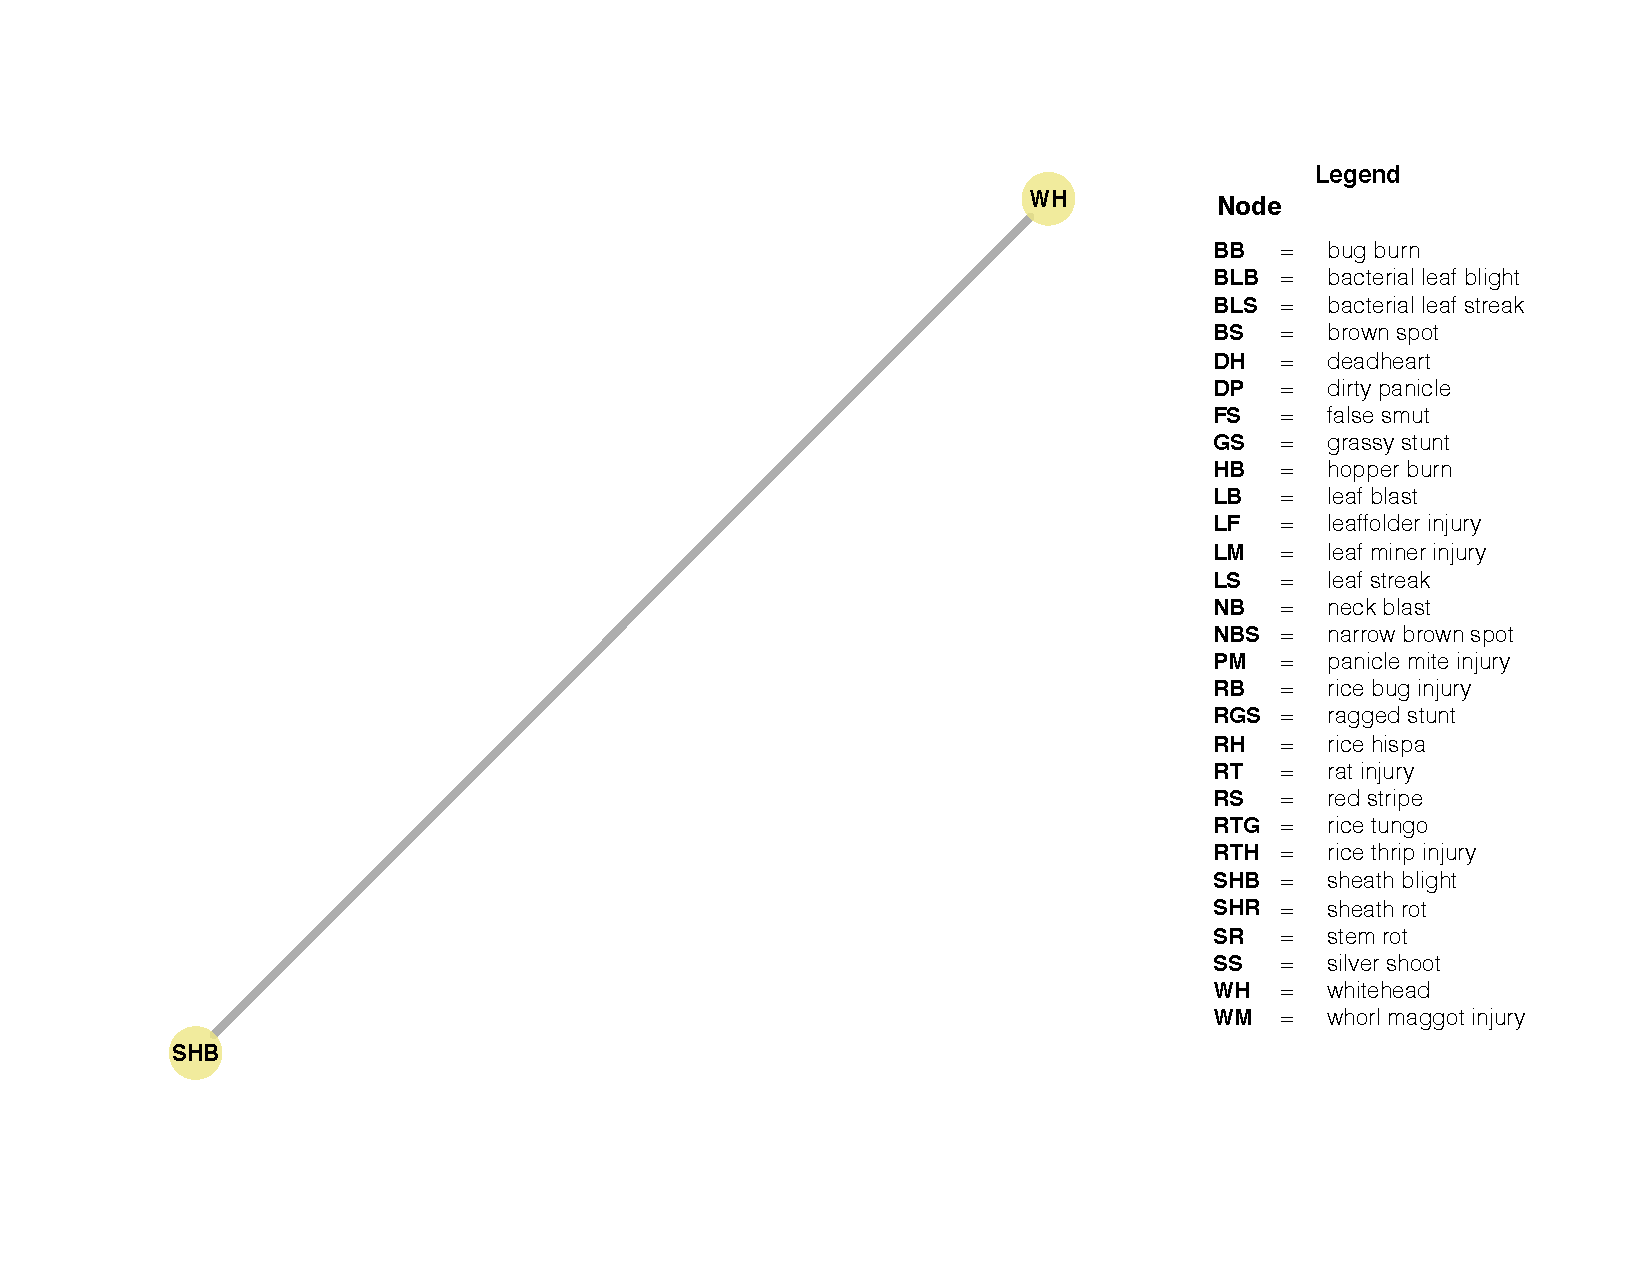
\includegraphics[width = 1\textwidth]{figures/difyieldTM.pdf}
        \caption{Differential co-occurrence network of rice injuries in different yield levels at Central Plain, Thailand. The layout of the network graph is based on the Fruchterman-Reingold algorithm, which places nodes with stronger or more connections closer to each other.}
        \label{fig:networkCP_ds}
    \end{subfigure}
    \begin{subfigure}[b]{1\textwidth}
        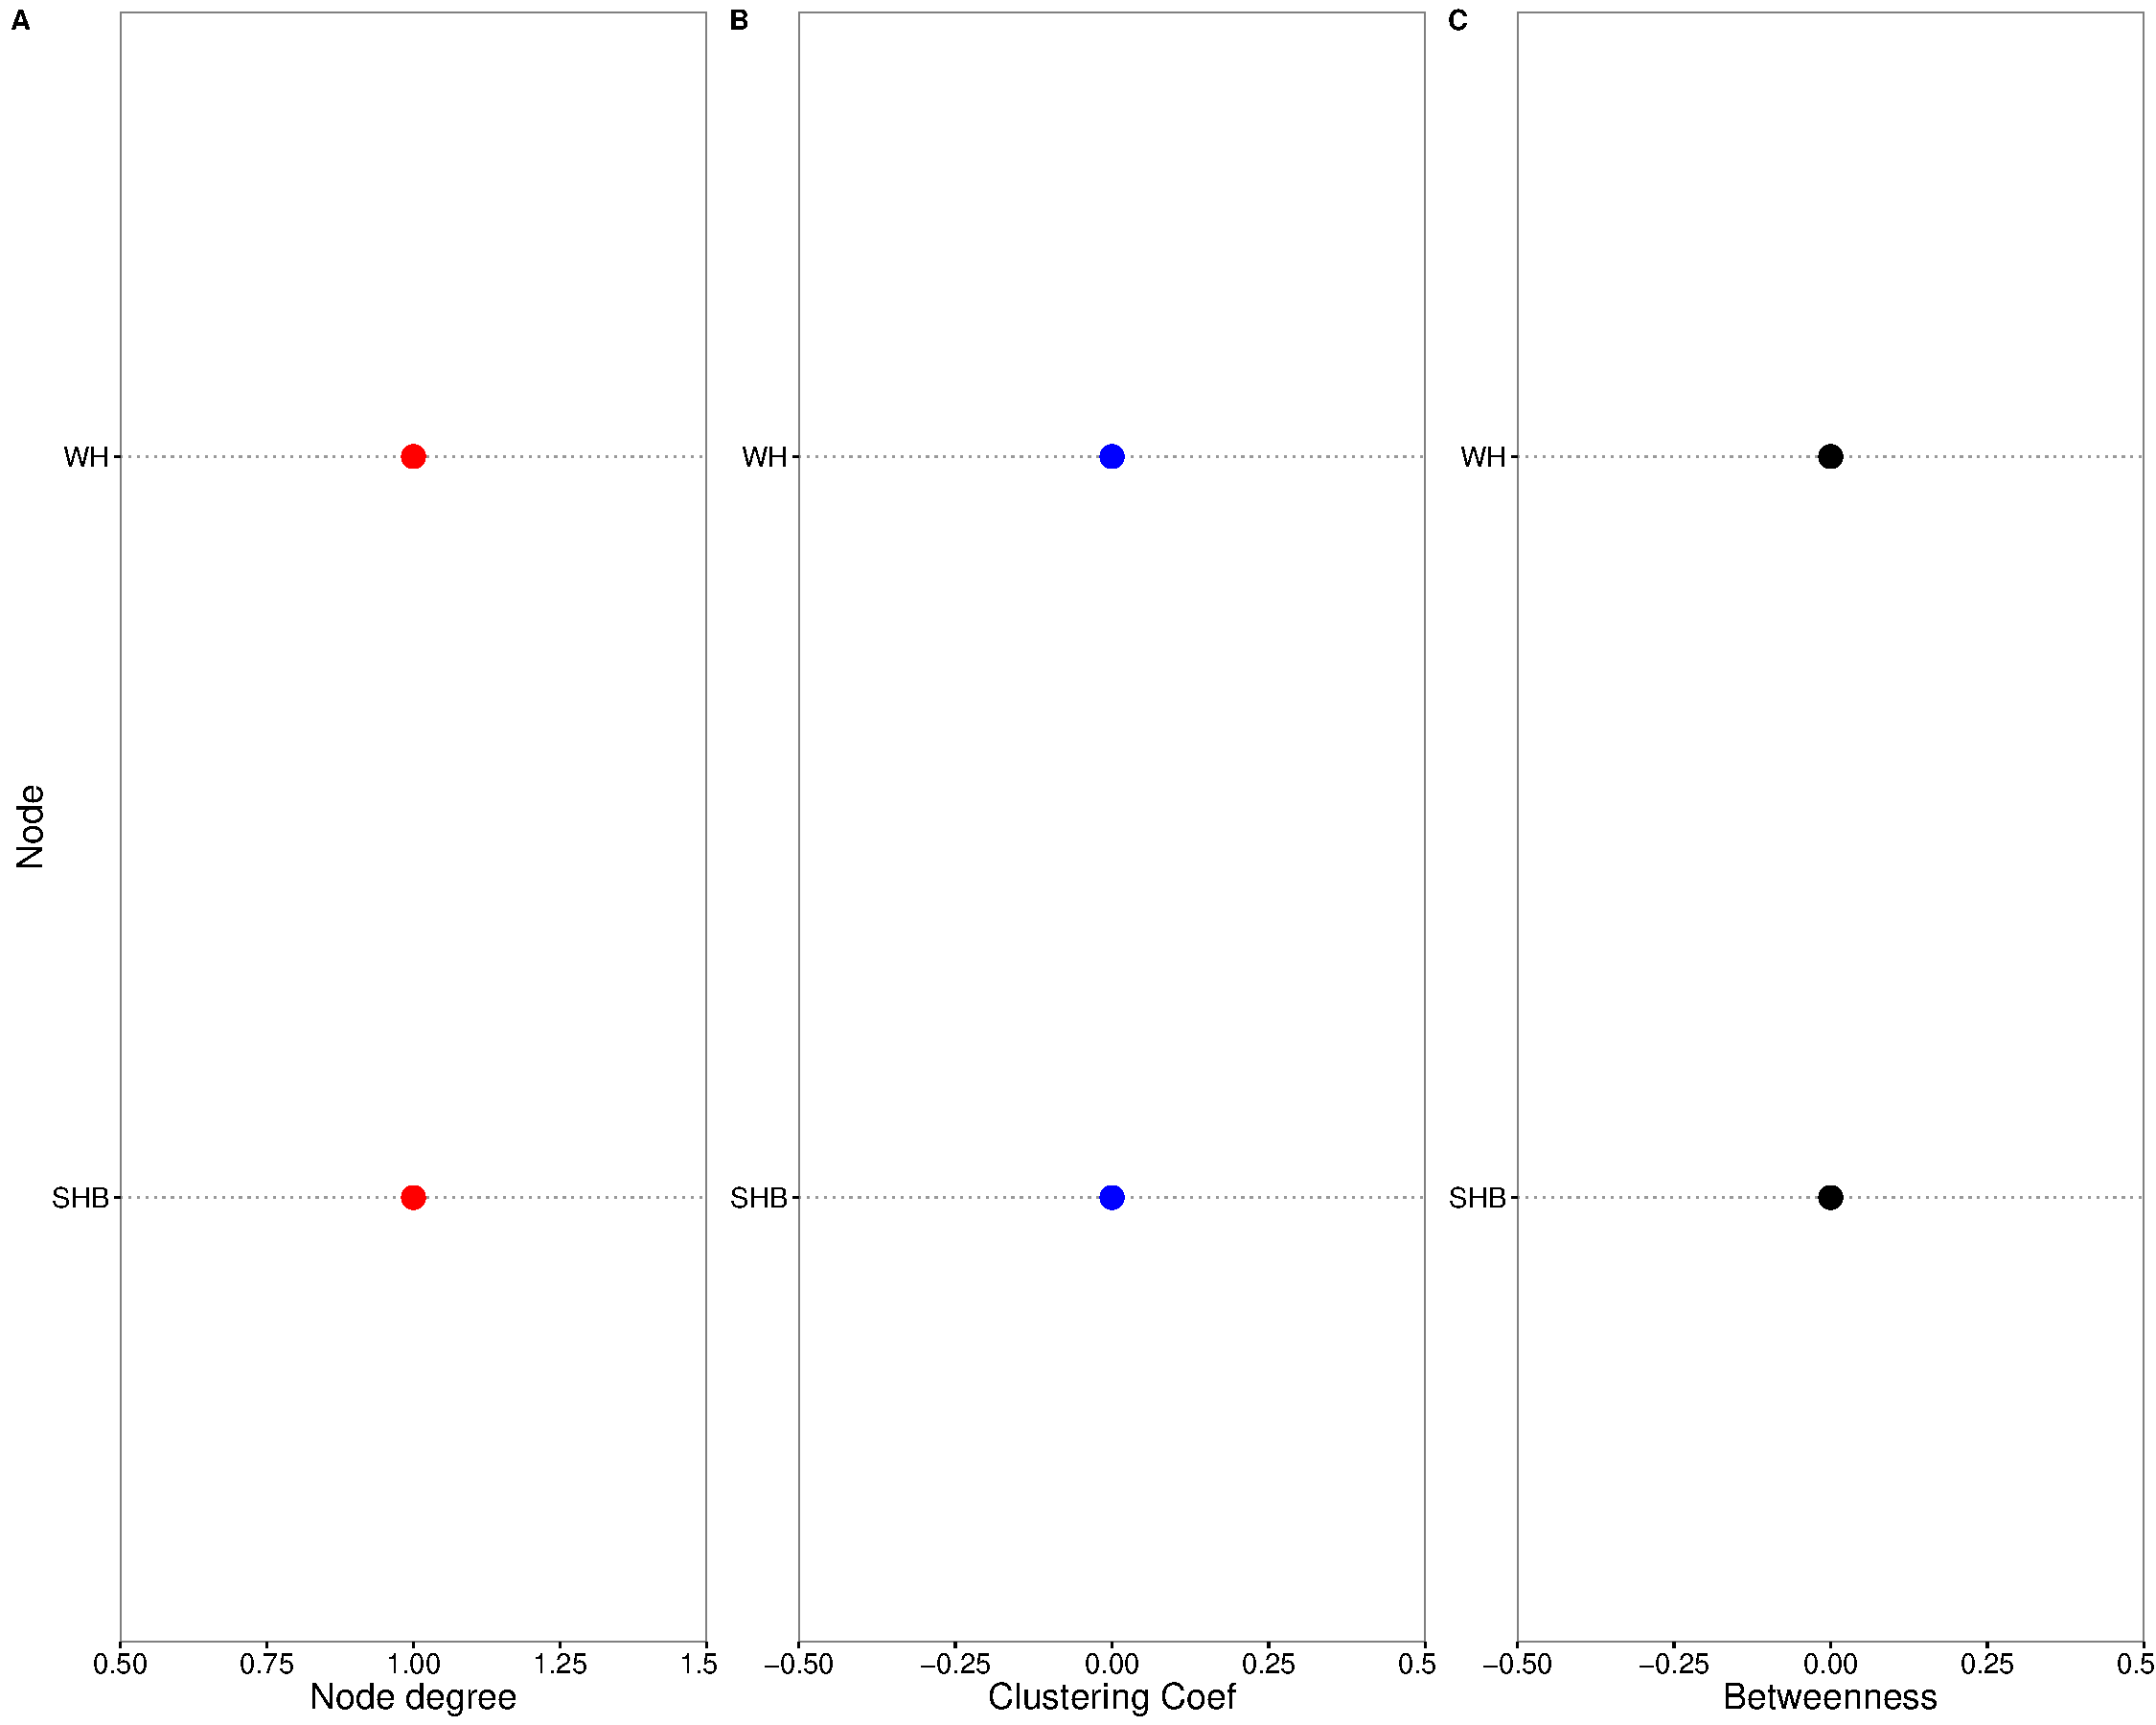
\includegraphics[width = 1\textwidth]{figures/yield_dif_nodepropTamil_Nadu.pdf}
        \caption{Three centrality measures of the nodes in co-occurrence network of rice injuries in dry season at Central Plain. A: node degree, B:clustering coefficient, and C:Betweenness.}
        \label{fig:nodepropdifyield_TM}
    \end{subfigure}
    \caption{Rice injuries in dry season in Central Plain, Thailand}
    \label{fig:CP_ds}
\end{figure}


\begin{figure}
    \centering
    \begin{subfigure}[b]{1\textwidth}
        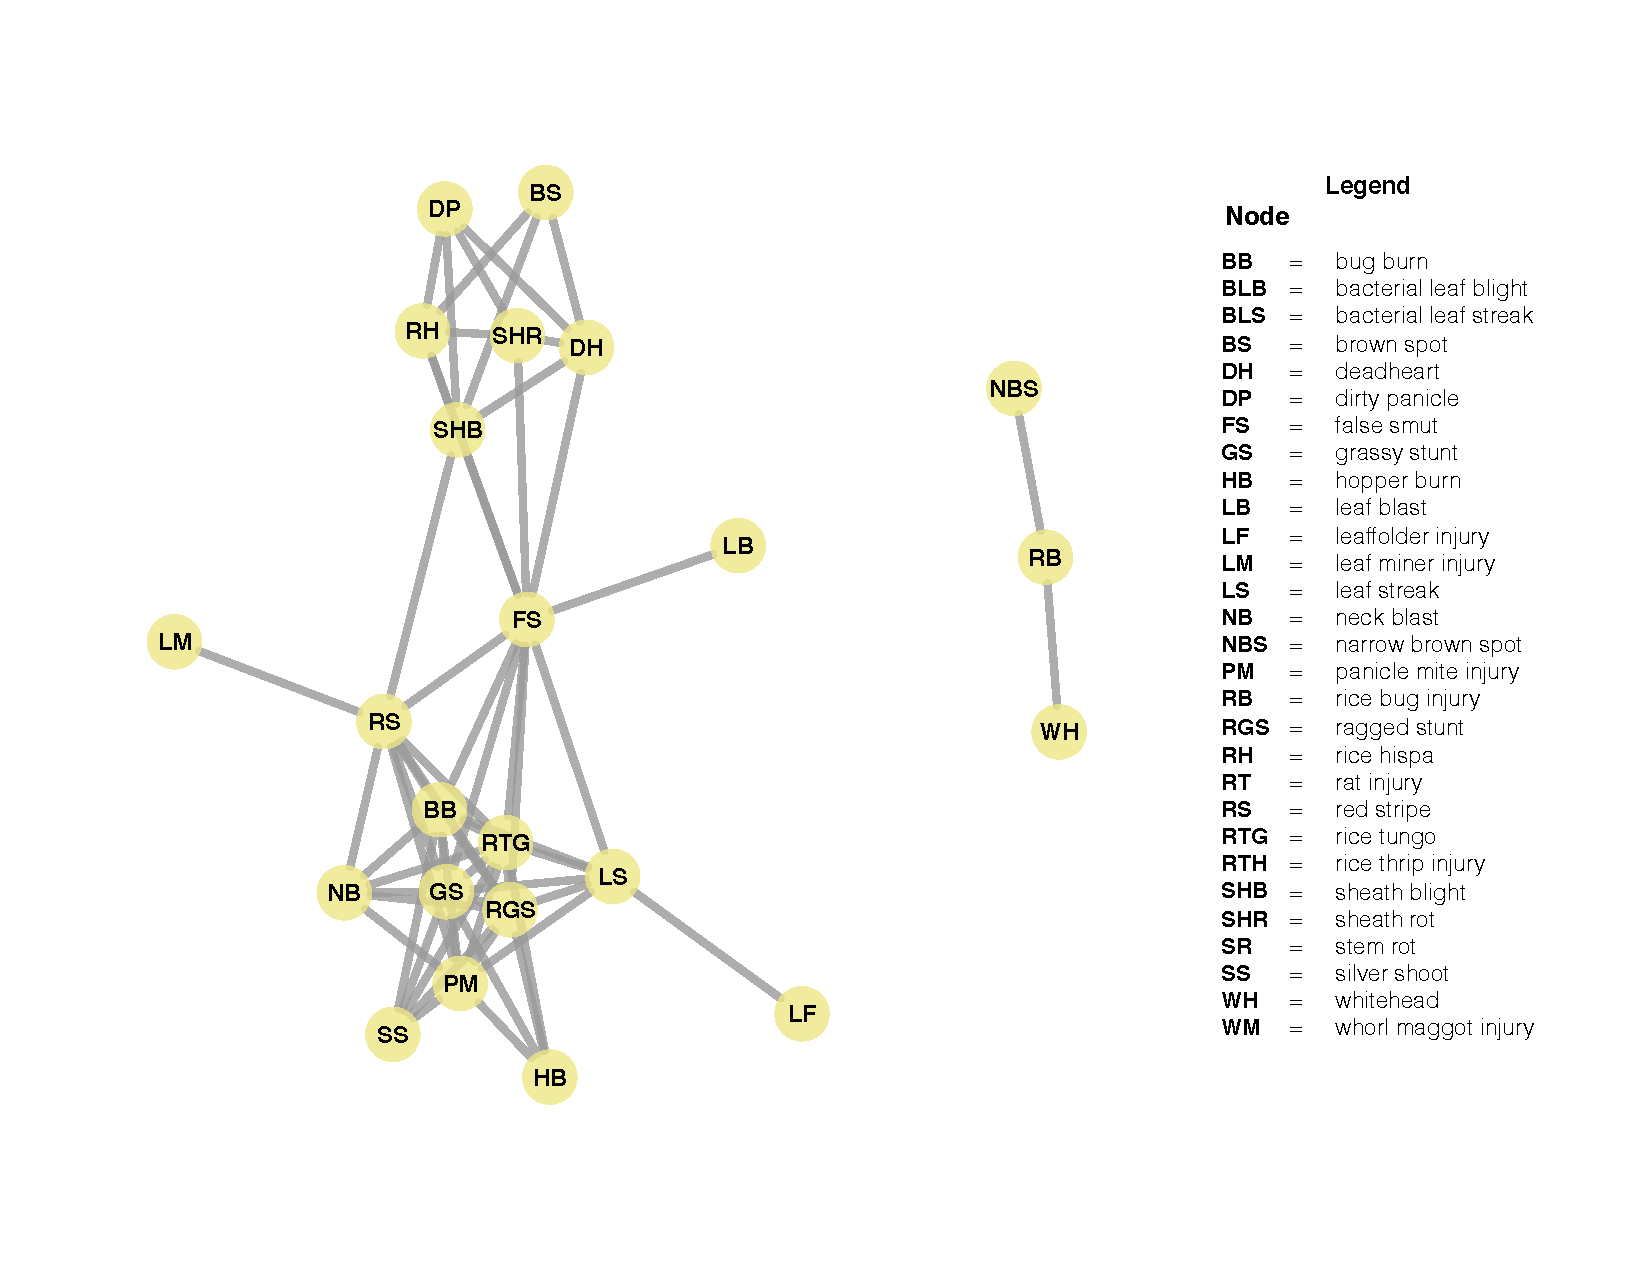
\includegraphics[width = 1\textwidth]{figures/difyieldWJ.pdf}
        \caption{Differential co-occurrence network of rice injuries in different yield levels at Central Plain, Thailand. The layout of the network graph is based on the Fruchterman-Reingold algorithm, which places nodes with stronger or more connections closer to each other.}
        \label{fig:networkCP_ds}
    \end{subfigure}
    \begin{subfigure}[b]{1\textwidth}
        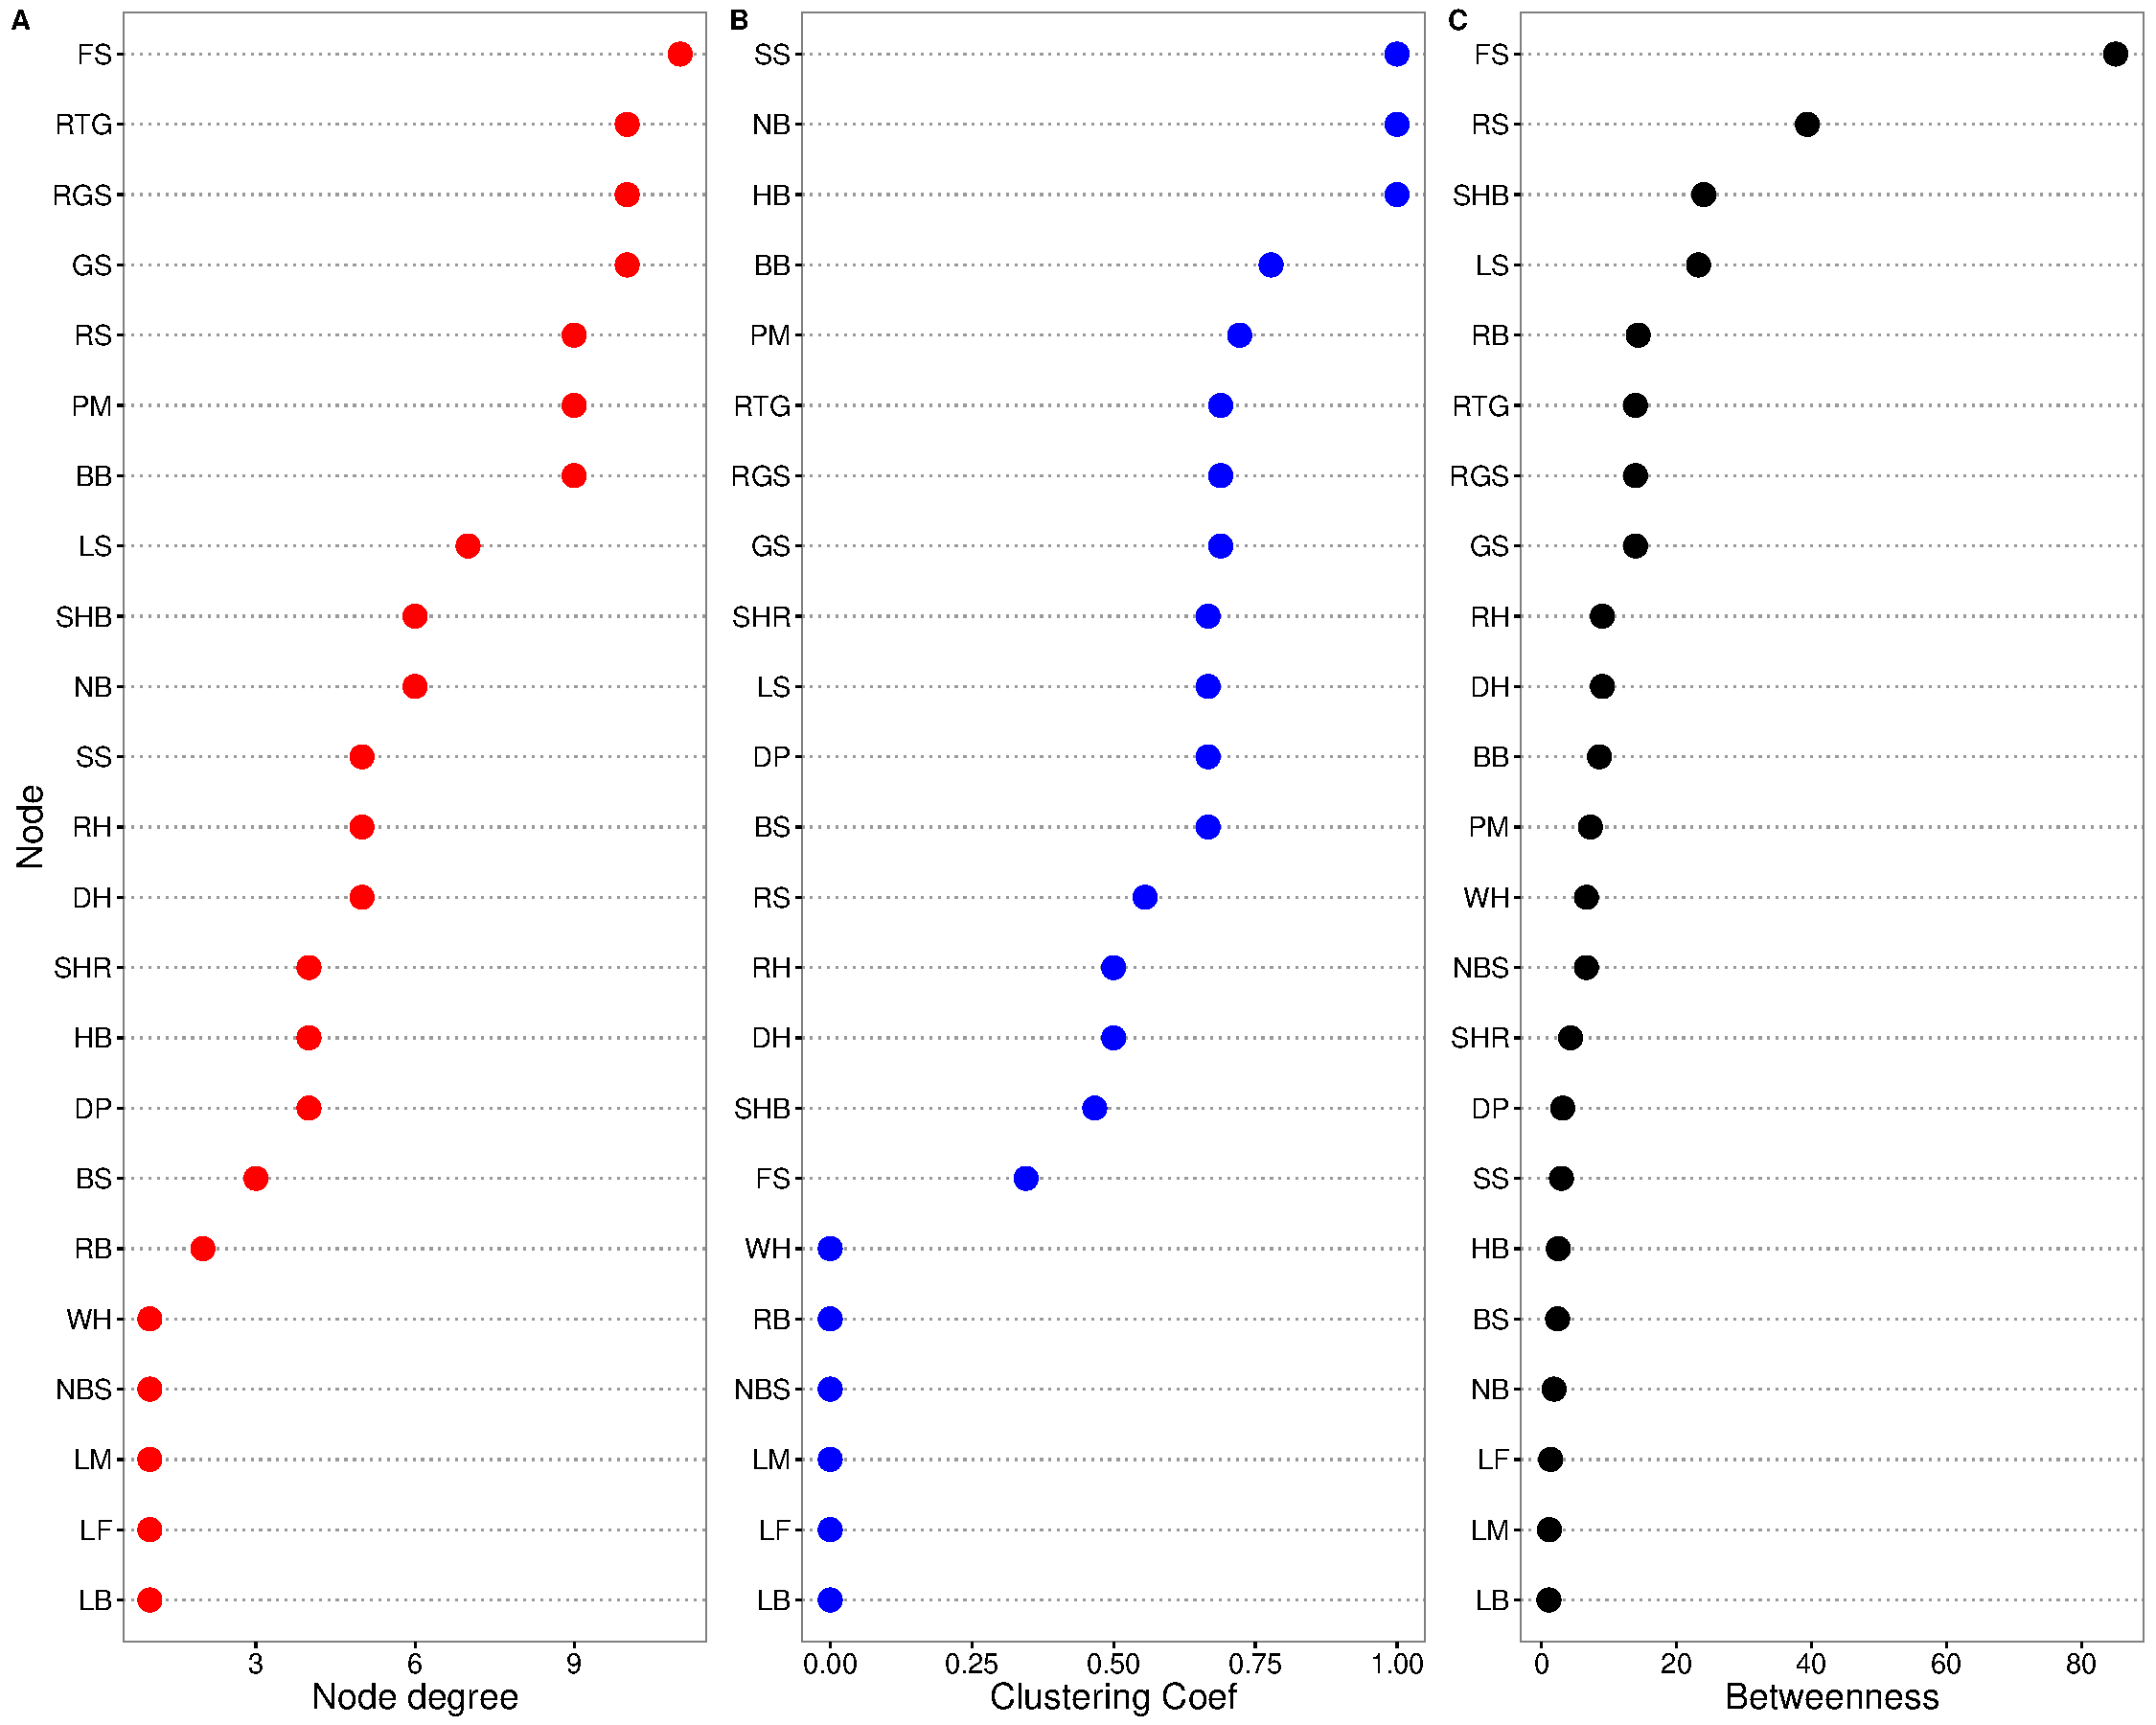
\includegraphics[width = 1\textwidth]{figures/yield_dif_nodepropWest_Java.pdf}
        \caption{Three centrality measures of the nodes in co-occurrence network of rice injuries in dry season at Central Plain. A: node degree, B:clustering coefficient, and C:Betweenness.}
        \label{fig:nodepropCP_ds}
    \end{subfigure}
    \caption{Rice injuries in dry season in Central Plain, Thailand}
    \label{fig:CP_ds}
\end{figure}
 